%%
%% TutQuartusSchematic - Schematic Entry Tutorial Using Quartus And ModelSim
%%
%% (c) J. op den Brouw <J.E.J.opdenBrouw@hhs.nl>
%%
%% v1.0, 26-aug-2014 - initial \LaTeX version Word 2003 v013
%% v1.1,    ??       -  ??
%% v1.2, 13-sep-2014 - changed to way footnotes are rendered.
%% V1.3
%% v1.4,  4-sep-2015 - changed item 4 in list ...
%% v1.5, 13-aug-2016 - changed logo to pdf version
%%                     first commit to BitBucket.
%% v1.6, 28-aug-2018 - changed to v13.0sp1 & v10.1d

\documentclass[a4paper,12pt,fleqn,twoside]{book}
\usepackage[utf8]{inputenc}
\usepackage[T1]{fontenc}

%% No double page clears...
\let\cleardoublepage\clearpage

\newif\ifbetaversion
\betaversiontrue

%% User's stuff
\def\tutauthor{J.E.J. op den Brouw}
\def\tuttitle{Tutorial Schematic Entry met\\ Quartus 13.0sp1\\ en\\ ModelSim-Altera 10.1d}
\def\tutpicscale{0.455}
\def\tutvak{INLDIG}
\def\tutkortnaam{Tutorial Quartus Schematic Entry}

%% Some nice defines.
%% My email address, nicely in a href
\newcommand\emailaddress{\href{mailto:J.E.J.opdenBrouw@hhs.nl}{\sffamily J.E.J.opdenBrouw@hhs.nl}}
%% Formatting of menu, buttons and names (e.g. file names)
\newcommand{\menu}[1]{\texttt{\textbf{#1}}}
\newcommand{\knop}[1]{\texttt{\textbf{#1}}}
\newcommand{\naam}[1]{\texttt{#1}}

%% maketitle stuff
\author{\tutauthor}
\title{\tuttitle}
\date{\today}

%% Use packages...
\usepackage{color}
\usepackage{array}
\setlength{\mathindent}{1em}

%% PDF Version and compression...
\pdfminorversion=5
\pdfobjcompresslevel=2

%% Dutch spelling of chapter, section, etc.
\usepackage[dutch]{babel}

%% Allows increasing the font size of specific fonts beyond LaTeX default specifications
\usepackage{anyfontsize}

%% Set page layout
%\usepackage[a4paper,bindingoffset=0.2in,left=.7in,right=0.7in,top=1in,
\usepackage[a4paper,bindingoffset=0.2in,left=0.8in,right=0.8in,top=1in,
%            bottom=1.1in,footskip=.40in,showframe]{geometry}
            bottom=1.1in,footskip=.40in]{geometry}

%% Include graphics files
\usepackage{graphicx}

%% Enumerate items
\usepackage{enumitem}

%% Using floats
\usepackage{float}

%% Array
\usepackage{array}

%% Tabu package for nice tables
\usepackage{tabu}

%% Use the AMS Mathematical characters
\usepackage{mathtools}
\usepackage{amsfonts}
\usepackage{amssymb}

%% The L Modern Font
%\usepackage{lmodern}
%% Sort of Arial
%\usepackage[scaled=.92]{helvet}
%\renewcommand{\familydefault}{\sfdefault}
%% Sort of Times New Roman
\usepackage{mathptmx}
%\usepackage[scaled=.98,sups,osf]{XCharter}% lining figures in math, osf in text
\usepackage{textcomp} 

%% Set paragraph skips et al.
\usepackage[parfill]{parskip}

%% Footnotes at the bottom of the page
% http://archive.cs.uu.nl/mirror/CTAN/macros/latex/contrib/footmisc/footmisc.pdf
% ruimte onder aan de pagina tussen tekst en voetnoot niet na voetnoot
\usepackage[bottom,hang,multiple]{footmisc}
% inspringen
\setlength{\footnotemargin}{1em}
% ruimte tussen footnotes:
\setlength{\footnotesep}{0.7\baselineskip}
%% Continuous footnote numbering
\usepackage{chngcntr}
\counterwithout{footnote}{chapter}

%% Lay things over a picture
\usepackage[abs]{overpic}

%% Enhanced plotting of picture environments
\usepackage{pict2e}

%% Use computer code listings
\usepackage{listings}
%\usepackage[scaled=0.90]{inconsolata}
\usepackage[scaled=0.80]{beramono}

%% Change the way chapters and sections are formatted.
\usepackage{titlesec}
\titleformat{\chapter}[hang] 
{\fontfamily{phv}\selectfont\Huge\bfseries\scshape}{\thechapter.}{0.5em}{}
\titleformat{\section}{\fontfamily{phv}\selectfont\large\bfseries}{\thesection}{1em}{}
\titleformat{\subsection}{\fontfamily{phv}\selectfont\bfseries}{\thesubsection}{1em}{}
\titlespacing*{\chapter}{0pt}{25pt}{15pt}
%\titlespacing*{\section}{0pt}{17pt}{3pt}
\titlespacing*{\section}{0pt}{1.44\baselineskip}{0.255\baselineskip}
%\titlespacing*{\subsection}{0pt}{12pt}{1pt}
\titlespacing*{\subsection}{0pt}{\baselineskip}{0.851\baselineskip}
\titlespacing*{\subsubsection}{0pt}{\parskip}{-\parskip}
%\titlespacing*{\subsubsection}{0pt}{\baselineskip}{-\baselineskip}
%%%\titlespacing*{\section}{0pt}{1.2\baselineskip}{.4\baselineskip}
%%%\titlespacing*{\subsection}{0pt}{.8\baselineskip}{.2\baselineskip}
%%%\titlespacing*{\subsubsection}{0pt}{.6\baselineskip}{0pt}


%% Making captions nicer...
\usepackage[font=footnotesize,format=plain,labelfont=bf,up,textfont=sl,up]{caption}
\captionsetup[table]{justification=raggedright,skip=0.1\baselineskip}
%\captionsetup[figure]{belowskip=-6pt}
\captionsetup[figure]{belowskip=-0.5\baselineskip}

%% Fancy headers and footers...
\usepackage{fancyhdr}
\pagestyle{fancy}
\fancyhead{} % clear all header fields
\renewcommand{\headrulewidth}{0pt} % no line in header area
\renewcommand{\footrulewidth}{0.4pt} % 0.4pt line
\fancyfoot{} % clear all footer fields
\fancyfoot[LE,RO]{\thepage}           % page number in "outer" position of footer line
%\fancyfoot[CE,CO]{\tutvak}
\fancyfoot[RE,LO]{\tutkortnaam} % other info in "inner" position of footer line
\makeatletter
\let\ps@plain\ps@fancy
\makeatother

%% List settings for VHDL code
\definecolor{dkgreen}{rgb}{0,0.6,0}
\definecolor{gray}{rgb}{0.5,0.5,0.5}
\definecolor{mauve}{rgb}{0.58,0,0.82}
\definecolor{lightgray}{rgb}{0.95,0.95,0.95}

%% Using hyperrefs...
\usepackage{hyperref}
\hypersetup{
	colorlinks=true,
	linkcolor=blue,
    pdftitle={\tuttitle},
    pdfauthor={\tutauthor},
    pdfsubject={},
    pdfkeywords={\tutkortnaam} {\tutvak}
}

%% Create our own maketitle macro
\makeatletter
\def\maketitle{%
  \null
  \thispagestyle{empty}%
  \vfill
  \begin{center}\leavevmode
    {\fontfamily{phv}\fontsize{35pt}{60pt}\selectfont\bfseries\scshape \@title\par}%
    \vskip 8.0cm
    \begin{minipage}[c]{.50\linewidth}
       
\includegraphics[width=\linewidth]{HHS_grijs_groen_fc}
    \end{minipage}\hfill
    \begin{minipage}[c]{0.40\linewidth}
       {\hfill \large \@author\par}%
       \vskip 0.03cm
       {\hfill \large De Haagse Hogeschool\par}%
       \vskip 0.03cm
       {\hfill \large Opleiding Elektrotechniek\par}%
       \vskip 0.03cm
       {\hfill \large \@date\par}%
       \vskip 0.03cm
       {\hfill \large \emailaddress\par}%
  \end{minipage}
  \end{center}%
  \vfill
  \null
  }
\makeatother

%% Def by Jean-Côme Charpentier
\lstdefinelanguage{tclfix}% from tcl definition
{alsoletter={.:,*=&-},%
morekeywords={after,append,array,names,exists,anymore,donesearch,%
get,nextelement,set,size,startsearch,auto_mkindex,binary,break,%
case,catch,cd,clock,close,concat,console,continue,default,else,%
elseif,eof,error,eval,exec,-keepnewline,exit,expr,fblocked,%
fconfigure,fcopy,file,atime,dirname,executable,exists,extension,%
isdirectory,isfile,join,lstat,mtime,owned,readable,readlink,%
rootname,size,stat,tail,type,writable,-permissions,-group,-owner,%
-archive,-hidden,-readonly,-system,-creator,-type,-force,%
fileevent,flush,for,foreach,format,gets,glob,global,history,if,%
incr,info,argsbody,cmdcount,commands,complete,default,exists,%
globals,level,library,locals,patchlevel,procs,script,tclversion,%
vars,interp,join,lappend,lindex,linsert,list,llength,lrange,%
lreplace,lsearch,-exact,-regexp,-glob,lsort,-ascii,-integer,%
-real,-dictionary,-increasing,-decreasing,-index,-command,load,%
namespace,open,package,forget,ifneeded,provide,require,unknown,%
vcompare,versions,vsatisfies,pid,proc,puts,-nonewline,pwd,read,%
regexp,-indices,regsub,-all,-nocaserename,return,scan,seek,set,%
socket,source,split,string,compare,first,index,last,length,match,%
range,tolower,toupper,trim,trimleft,trimright,subst,switch,tell,%
time,trace,variable,vdelete,vinfo,unknown,unset,uplevel,upvar,%
vwait,while,acos,asin,atan,atan2,ceil,cos,cosh,exp,floor,fmod,%
hypot,log,log10,pow,sin,sinh,sqrt,tan,tanh,abs,double,int,round,%
foreach_in_collection,post_message,-submsgs,add,wave,vsim,vcom,%
vlib,vmap,vdel,transcript,view,run
},%
morestring=[d]",%
% MoreSelectCharTable=% <= the strange definition
% \lst@CArgX\#\relax\lst@DefDelimB{}{}%
% {\ifx\lst@lastother\lstum@backslash
% \expandafter\@gobblethree
% \fi}%
% \lst@BeginComment\lst@commentmode
% {{\lst@commentstyle}\lst@Lmodetrue}%
morecomment=[l]\# % <= this one ! Much simpler
}[keywords,comments,strings]%

\lstset{
  basicstyle=\linespread{0.92}\small\ttfamily,
  commentstyle=\itshape,
  numbers=left,
  numberstyle=\tiny\color{gray},
  stepnumber=1,
  numbersep=5pt,
  backgroundcolor=\color{lightgray},
  showspaces=false,
  showstringspaces=false,
  showtabs=false,
  frame=lines,
  rulecolor=\color{black},
  tabsize=4,
  captionpos=b,
  breaklines=true,
  breakatwhitespace=false,
  title=\lstname,
  upquote=true,
}

%% Needed
\usepackage{calc}
%% Framed high lighted text
\def\fpf#1{%
	\medskip%
	%\fbox{\parbox{0.985\textwidth}{\vspace*{\medskipamount}\centering\textbf{#1}\vspace*{\medskipamount}}}%
	\fbox{\parbox{\textwidth-\marginparsep}{\vspace*{\medskipamount}\centering\textbf{#1}\vspace*{\medskipamount}}}%
	\medskip%
}

%% \raisebox{...}
\def\rb#1{\raisebox{-0.23ex}{#1}}

%% An arrow
\def\pijl{$\rightarrow$}%

\begin{document}

\raggedbottom

\maketitle

\tableofcontents
\vfill

Voor suggesties en/of opmerkingen over deze tutorial kan je je wenden tot
J. op den Brouw, kamer D1.047, of je kunt email versturen naar \emailaddress.


%% Print list of figs and list of listing on one page
\newpage
\listoffigures
\begingroup
\let\cleardoublepage\relax
\listoftables
\lstlistoflistings
\endgroup



\chapter{Inleiding}
\label{chap:inleiding}
Vroeger was het de gewoonte om schakelingen op te bouwen uit losse componenten
zoals transistoren, weerstanden en condensatoren. Naarmate de schakelingen
complexer werden nam echter de kans op slechte verbindingen toe en de
betrouwbaarheid af. Daarom is men er toe over gegaan meerdere componenten op
\'{e}\'{e}n siliciumchip te integreren; voor digitale schakelingen begon dit
met poorten en flipflops (Small Scale Integration), ging verder  met tellers,
decoders, multiplexers et cetera (Medium Scale Integration), en het einde is
met de geavanceerde microprocessors en geheugens nog niet in zicht (Very Large
Scale Integration). Het inwendige van zo'n ge\'{e}ntegreerde schakeling is
echter niet te veranderen; de functionaliteit ligt vast. Een nieuwe generatie
van componenten, de zogenaamde configureerbare logica, biedt de mogelijkheid
zelf een schakeling te ontwikkelen. Deze componenten bevatten een groot aantal
basisschakelingen (poorten, flipflops en losse verbindingen) die door de
gebruiker willekeurig met elkaar en met in- en uitgangspennen kunnen worden
verbonden. Bovendien zijn er recepten om bijvoorbeeld in \'{e}\'{e}n klap een
gehele 16-bit teller te configureren (bibliotheekelementen). De taak van een
ontwerper verschuift dus van solderen naar beschrijven.

Hoe gaat dit nu in zijn werk? Het eigenlijke beschrijven gebeurt met behulp van
een PC. Dit is dus de onmisbare schakel in het geheel. De ontwerper bedenkt
eerst een schakeling op papier. Als het probleem niet in \'{e}\'{e}n keer te
overzien  is, worden er deelontwerpen gemaakt die onderling verbonden zijn. Elk
deelontwerp bevat een schakeling of, als het probleem nog niet te overzien 
is, weer deelontwerpen. We noemen dit principe hi\"{e}rarchisch ontwerpen.

Nadat alle deelontwerpen zijn bedacht wordt overgegaan tot het invoeren van de
deelschakelingen. Hier hebben we een verscheidenheid aan keuzes. We kunnen
schakelingen invoeren als een schema met behulp van een tekenpakket, maar ook
met behulp van een speciale taal die beschrijft wat de schakeling moet doen,
bijvoorbeeld VHDL. Daarnaast zijn er nog invoermogelijkheden via
toestandsmachines, booleaanse functies en waarheidstabellen.

Wanneer alle deelontwerpen gemaakt zijn, moeten ze worden omgezet naar een
bestand met gegevens die in de component geladen moet worden. Dit proces heet
synthetiseren. Als tijdens dit omzetten een fout wordt geconstateerd,
bijvoorbeeld twee uitgangen aan elkaar, wordt dit gemeld aan de ontwerper en
moet de fout hersteld worden. Treden er geen fouten op dan levert de software
een bruikbaar configuratiebestand op. LET OP: dit betekent nog niet dat het
ontwerp precies doet wat het moet doen! Er kan nog best een functionele fout
in het ontwerp zitten. Denk hierbij aan een programmeertaal. De compiler vindt
geen syntax-fouten maar dat geeft geen garantie dat het programma doet wat het
moet doen.

De laatste stap is het daadwerkelijk configureren van de component. Daarvoor is
een hardware-programmer nodig. Die zorgt ervoor dat het configuratiebestand in
de configureerbare component wordt gestopt.

\newpage
Het ontwerptraject (een af te leggen weg van handelingen) wordt nu als volgt:

\begin{itemize}\itemsep-1pt
\item bedenken van de schakeling,
\item invoeren van het ontwerp met poorten,
\item functionele simulatie
\item omzetten van de poortschakeling naar een voor de configureerbare
      component geschikt bestand, eventuele fouten moeten eerst aangepast
      worden,
\item eventueel timing simulatie
\item testen van de schakeling.
\end{itemize}

In figuur~\ref{fig:009designflow} is het ontwerptraject nog eens schematisch
aangegeven.
 
\begin{figure}[H]
\centering
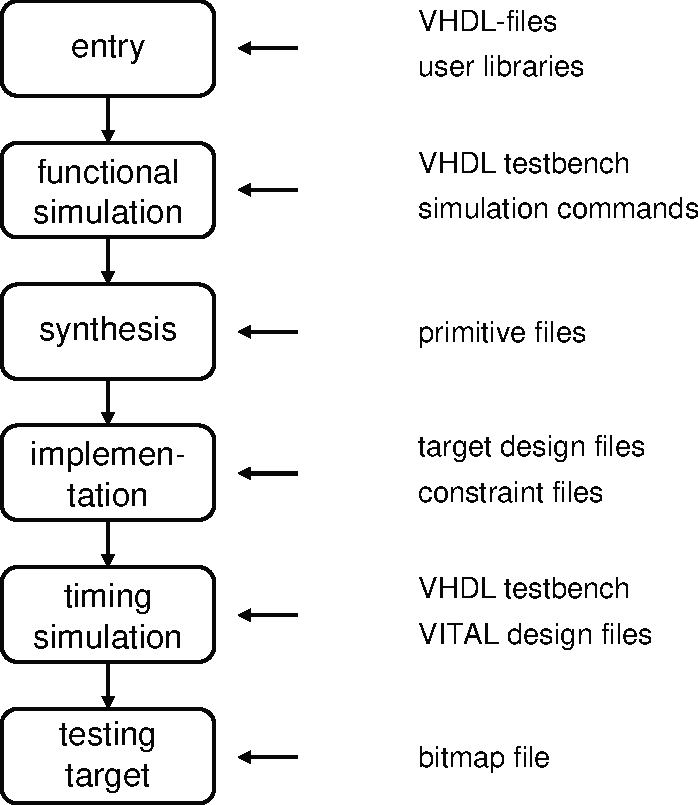
\includegraphics[scale=0.63]{009designflow.pdf}
\caption{Het ontwerptraject.}
\label{fig:009designflow}
\end{figure}

Het bedenken van de schakeling is een creatief proces. Ervaring en goede kennis
van digitale systemen helpt je hierbij op weg. Het opzetten van een goede
simulatie hoort bij de vaardigheden van de ontwerper. De rest wordt eigenlijk
door de tools van Quartus afgehandeld. Het is voor de ontwerper niet meer
interessant om op laag niveau de hardware te bekijken. Je moet er dan
wel zeker van zijn dat je de hardware met de juiste regels beschreven hebt:
combinatoriek en flankgevoelige geheugenelementen. Latches zijn uit den boze.


\chapter{Practicumomgeving}
\label{chap:practicumomgeving}
In dit hoofdstuk wordt de practicumomgeving toegelicht.


\section{Ontwikkelbord}
\label{sec:ontwikkelbord}
Het practicum maakt gebruik van een ontwikkelbordjes, de DE0. Op dit bordje
is een FPGA van Altera geplaatst. Hieronder is een foto weergegeven.

\begin{figure}[H]
\centering
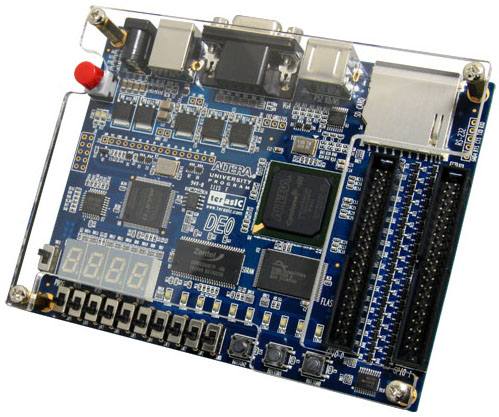
\includegraphics[scale=0.63]{image-de0.jpg}
\caption{Het DE0-ontwikkelbord}
\label{fig:image-de0}
\end{figure}
 
Daarnaast zijn ook nog schakelaars, leds en 7-segment displays aanwezig. Zie
hoofdstuk \ref{chap:ontwikkelbordje} voor meer informatie.

Naast het bordje wordt een softwarepakket van de fabrikant gebruikt genaamd
Quartus II. In de volgende paragraaf wordt een korte beschrijving gegeven van
de software. Je hoeft niet alles in \'{e}\'{e}n keer te kennen. Verderop in
deze handleiding is een tutorial opgenomen die je stap voor stap door het
ontwerptraject loodst.

Om de component te configureren is een (hardware-)programmer nodig. Deze is op
het ontwikkelbord geplaatst. Er is alleen een USB-kabel nodig voor een
verbinding tussen een PC en het ontwikkelbord.

\subsubsection{Quartus II}
Quartus II is een alles-in-\'{e}\'{e}n pakket voor het ontwikkelen van digitale
schakelingen en het configureren van (Altera) componenten. Het bestaat uit een
viertal delen:

\begin{itemize}\itemsep-1pt
\item het invoergedeelte - d.m.v. schema's, VHDL, toestandsdiagrammen
\item synthesizer - dit deel vertaalt de invoer naar een netlist,
\item implemention - genereert een bit-file die je in de component kunt laden,
\item programmer - dit deel configureert de component via de USB-interface.
\end{itemize}

\subsubsection{ModelSim}
ModelSim is een VHDL-simulator die direct vanuit de broncode simuleert. Er zijn
in principe geen tussenstappen nodig zoals synthese. Je kan echter ook de
uitvoer van de synthese simuleren. Hierdoor krijg je inzicht in de
vertragingstijden. Met ModelSim is het mogelijk abstracte beschrijvingen van
digitale schakelingen te simuleren. Deze schakelingen zijn niet
synthetiseerbaar.

ModelSim kan als stand-alone pakket gebruikt worden. Wij zullen ModelSim
gebruiken als onderdeel van Quartus en ModelSim starten vanuit Quartus.


\section{Software-versies en web-edition}
\label{sec:softwareversies}
Het Quartus-pakket komt in twee smaken. Er is een volledige betaalde versie
waarbij een licentie-server nodig is en er is een zogenaamde \textsl{Web
Edition}. De
eerstgenoemde is de meest krachtige versie: alle \textsl{devices} van Altera
zijn hiermee te configureren. Daarnaast heb je hier nog optie-pakketten voor
DSP-ontwikkeling en digitale filters. De Web Wdition is gratis, heeft geen 
licentie-server nodig, maar kan niet synthetiseren voor alle beschikbare IC's.
Er zijn geen optie-pakketten beschikbaar.

Van ModelSim bestaan ook twee versies: de volledige, betaalde Altera-versie en
de zogenaamde \textsl{Altera Starter Edition}. De typering "Altera" geeft aan
dat het specifiek ontwikkeld is om met Quartus samen te werken. De betaalde
versie heeft geen beperkingen, de Altera Starter Edition kan maximaal 10000
VHDL-coderegels simuleren en verwerkt de code langzamer dan de betaalde versie.

De Web Edition van Quartus (met ModelSim ge\"{\i}ntegreerd) kan gevonden
worden op

%\hspace*{1cm}\url{https://www.altera.com/download/software/quartus-ii-we}
\hspace*{1cm}\url{http://dl.altera.com/13.0sp1/?edition=web#tabs-1}

%De Starter Edition van ModelSim kan gevonden worden op
%
%\hspace*{1cm}\url{https://www.altera.com/download/software/modelsim-starter}

De software draait op Windows\texttrademark\ \'{e}n Linux\texttrademark\ , er
is geen OS X-versie. Op het practicum wordt Windows gebruikt.

Let erop dat het practicum wordt uitgevoerd met versie 13.0sp1 resp\@. versie
10.1d.

Noot: aangeraden wordt om versie 13.0sp1 te installeren. Hogere versies
ondersteunen de FPGA's (Cyclone II en III) op de gebruikte ontwikkelbordjes
niet. Versie 13.0sp1 is prima geschikt om deze tutorial te doorlopen.
% Let er
%op dat de pictogrammen kunnen afwijken t.o.v.\@ versie 11.1sp1. De in
%het practicum gemaakte Quartus-projecten
%kunnen zonder problemen door zowel versie 13.0sp1 als 11.1sp1 geopend worden.
%Vanaf versie 13.0 is ModelSim ge\"{\i}ntegreerd in het installatiepakket.

\textbf{
Let op: versie 14.0 en hoger kunnen niet gebruikt worden i.s.m.\@ het
DE0-bordje!
}



\chapter{Ontwikkelbordje}
\label{chap:ontwikkelbordje}
In dit hoofdstuk wordt het ontwikkelbordje nader beschreven. Eerst wordt een
blokschema getoond en worden de diverse onderdelen kort beschreven. Daarna
volgt een paragraaf over de configureerbare component, de Altera Cyclone III,
met specificaties van het gebruikte type.


\section{Blokschema}
\label{sec:blokschema}
Het ontwikkelbord is ontwikkeld door het bedrijf Terasic in samenwerking met
Altera, de fabrikant van de Cyclone III. Een gedetailleerde beschrijving is
niet nodig; we geven slechts een blokschema van de onderdelen. Alles wat je
nodig hebt tijdens het practicum staat hier beschreven. In
figuur~\ref{fig:DE0-layout-yellow-1000} is een foto afgebeeld met de diverse
onderdelen.

%% Moet misschien nog iets groter.
\begin{figure}[H]
\centering
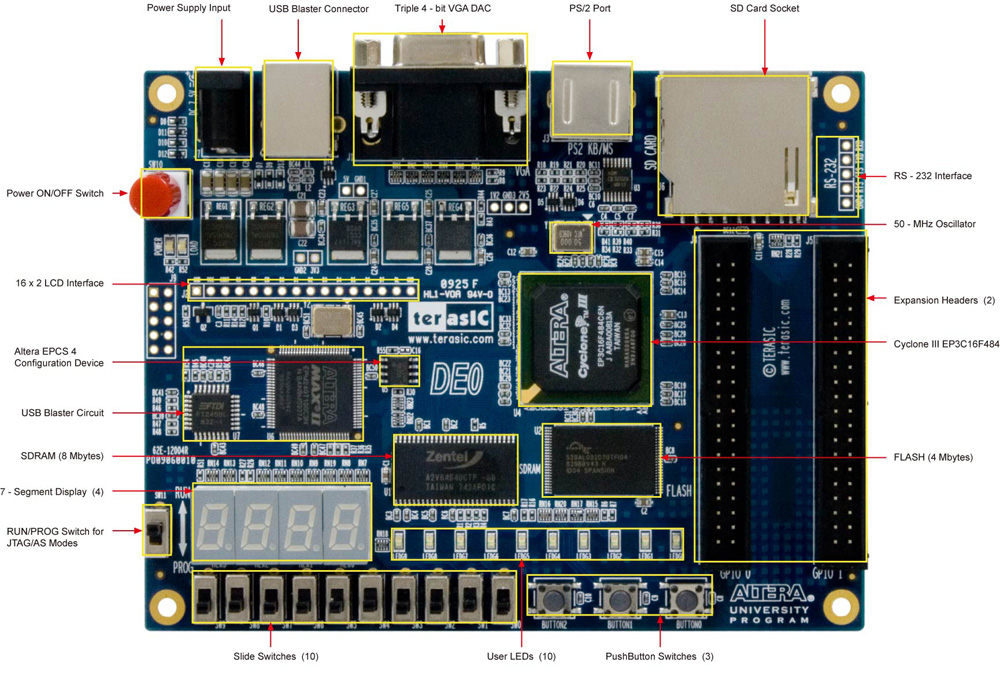
\includegraphics[scale=0.92]{DE0_layout_yellow_1000.jpg}
\caption{Het DE0-ontwikkelbord met benoeming van periferie}
\label{fig:DE0-layout-yellow-1000}
\end{figure}

In figuur~\ref{fig:010blockdiagram} is een blokschema weergegeven. Bij elk
onderdeel staat vermeld met hoeveel signalen het onderdeel verbonden is met de
Cyclone III. De voedingslijnen zijn niet meegenomen. 

\begin{figure}[H]
\centering
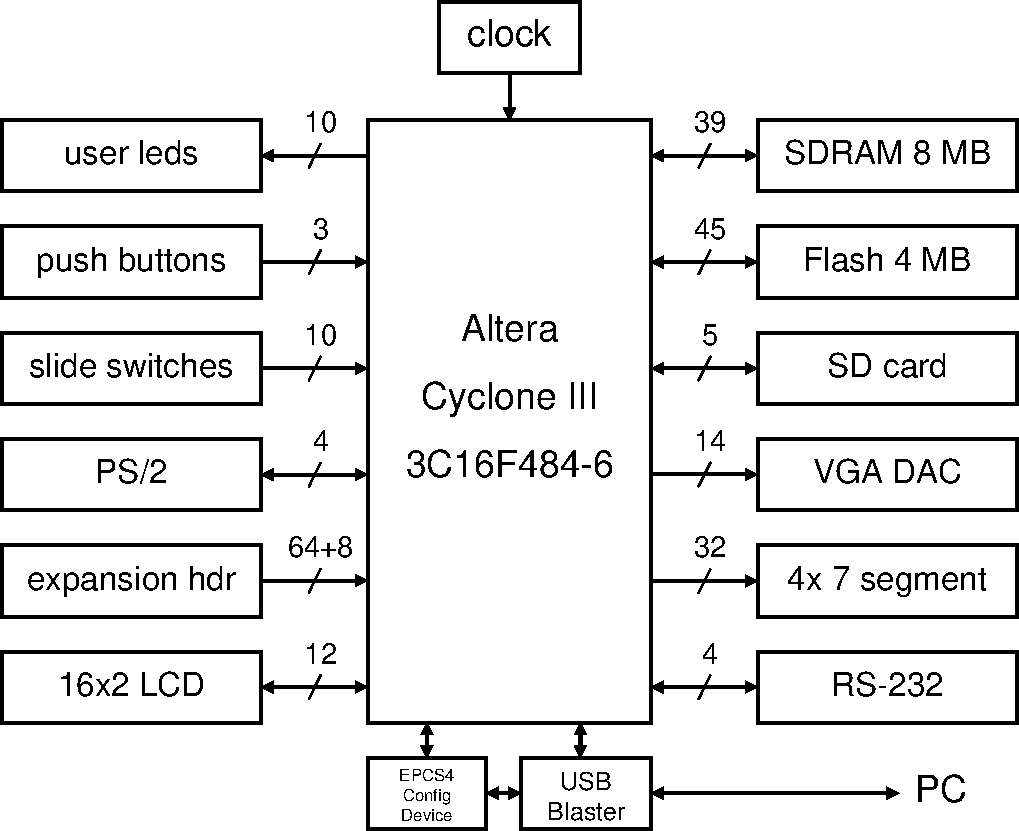
\includegraphics[scale=0.50]{010blockdiagram.pdf}
\caption{Blokschema ontwikkelbord}
\label{fig:010blockdiagram}
\end{figure}

\subsubsection{Cyclone III}
Het hart van het ontwikkelbord wordt gevormd door de Cyclone III EP3C16F484-6N
(zie figuur~\ref{fig:ep3c16f484c6n}). Dit is een configureerbaar IC waarin een
digitale schakeling kan worden geplaatst.

\begin{figure}[H]
\centering
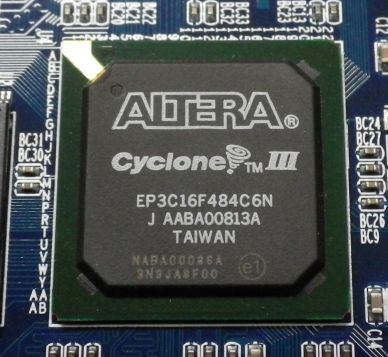
\includegraphics[scale=0.40]{ep3c16f484c6n.jpg}
\caption{Foto Cyclone III}
\label{fig:ep3c16f484c6n}
\end{figure}
%Figuur 3-3  -  foto EP3C16F484C-6N

\subsubsection{Push buttons}
Het ontwikkelbord heeft drie drukknoppen genaamd \naam{BUTTON2} t/m
\naam{BUTTON0}. Deze drukken geven een laag logisch
niveau (0) af als de knop is ingedrukt en een hoog logisch niveau (1) als de
knop niet is ingedrukt. Verder zijn deze drie knoppen ontdenderd en zijn te
gebruiken als kloksignaal.

\subsubsection{Slide switches}
Het ontwikkelbord heeft tien schuifschakelaars genaamd \naam{SW9} t/m
\naam{SW0}. Een schakelaar geeft een laag
logisch niveau (0) af als de schakelaar naar beneden is geschoven (het dichtst
bij de rand van de print) en een hoog logisch niveau (1) als de schakelaar naar
boven is geschoven. Deze schakelaars zijn niet ontdenderd en zijn alleen voor
niveaugevoelige ingangen bedoeld.

\subsubsection{Leds}
Het ontwikkelbord heeft tien groene leds \naam{LEDG9} t/m \naam{LEDG0}. Een
led brandt als een hoog logisch niveau (1) wordt aangeboden en is uit als een
laag logisch niveau (0) wordt aangeboden.

\subsubsection{7-segment displays}
Het ontwikkelbord heeft vier 7-segment displays waarmee getallen van
verschillend formaat kunnen worden gemaakt. Elk display bestaat uit zeven leds
waarmee een cijfer kan worden gevormd. Daarnaast heeft elk display een punt.
Een led brandt als een laag logisch niveau (0) wordt aangeboden en is uit als
een hoog logisch niveau (1) wordt aangeboden.

\subsubsection{Clock}
Het ontwikkelbord heeft \'{e}\'{e}n 50 MHz klokoscillator aan boord. Het
kloksignaal kan dienen als (direct) kloksignaal voor het klokken van flipflops
of als invoer voor een Phase Locked Loop (PLL).

Een overzicht van de pinaansluitingen en de layout van de 7-segment displays
is te vinden in bijlage~\ref{chap:pinbenaming}.

\subsubsection{Overige aansluitingen}
Het ontwikkelbord bevat verder nog een 8 MD SDRAM, een 4 MB Flash, een
VGA-uitgang, een LCD-interface, een SD-card interface, een PS/2-interface, een
RS-232-interface en een expansion header met 64 I/O-lijnen en 8 kloklijnen. Dit
wordt verder niet besproken.


\section{Altera Cyclone III}
\label{sec:alteracycloneiii}
De Cyclone III FPGA (Field Programmable Gate Array)\footnote{Het is wel raar
dat een FPGA configureerbaar heet, terwijl de naam suggereert dat ze
programmeerbaar zijn.} is opgebouwd uit zogenaamde logische elementen (Logic
Elements, LE). Met deze elementen kan je een digitale schakeling bouwen. Het 
gebruikte type heeft er 15408 aan boord. Om een indruk te geven wat dat
inhoudt: een volledige 32-bits processor (NIOS/II) gebruikt zo'n 1800
elementen. Je kan er dus acht processoren in kwijt.

In tabel~\ref{tab:gegevenscyclone} zijn wat gegevens te vinden.
\begin{table}[H]
\caption{Enige gegevens over de EP3C16F484C-6N}
\label{tab:gegevenscyclone}
\centering
\begin{tabular}{|l|l|}
\hline 
Aansluitpinnen (user I/O) & 484 (347) \\ 
\hline 
Logische elementen & 15408 \\ 
\hline 
Geheugenelementen & 15408 (\'{e}\'{e}n per element) \\ 
\hline 
RAM-bits & 516096 \\ 
\hline 
Vermenigvuldigers & 112 (9x9 bit) / 56 (18x18 bit) \\ 
\hline 
Phase Locked Loops & 4 \\ 
\hline 
Global Clock Networks & 20 \\ 
\hline 
$t_{PD(pin-to-pin)}$ & 6 ns \\ 
\hline 
$f_{MAX}$ (I/O, stand alone) & 250 MHz \\ 
\hline 
\end{tabular} 
\end{table}

Figuur~\ref{fig:003chip} geeft een Floor Plan van de bij de workshop gebruikte
3C16. Daarnaast heeft elke Cyclone RAM en vermenigvuldigers aan boord. De
vermenigvuldigers zijn sneller dan wanneer ze met LE's worden opgebouwd.
Je kan ze bijvoorbeeld gebruiken bij digitale signaalbewerking.

\begin{figure}[H]
\centering
%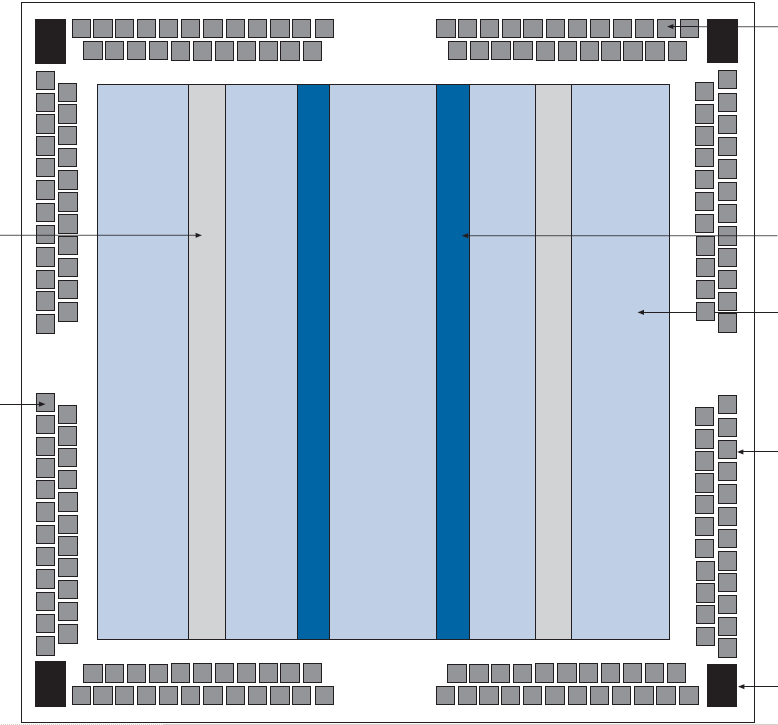
\includegraphics[scale=0.45]{003chip.png}
\begin{overpic}[scale=0.45,unit=1mm]{003chip}
\linethickness{1pt}
\put(-2,51){\makebox(0,0)[r]{\scriptsize 347 user I/O}}
\put(-2,78){\makebox(0,0)[r]{\scriptsize 504 kB embedded memory}}
\put(125,6){\makebox(0,0)[l]{\scriptsize configurable PLL}}
\put(125,43.5){\makebox(0,0)[l]{\scriptsize 250 MHz I/O access}}
\put(125,65.5){\makebox(0,0)[l]{\scriptsize 15048 LE's / 963 LAB's}}
\put(125,77.5){\makebox(0,0)[l]{\scriptsize 112 embedded multipliers}}
\put(125,110.7){\makebox(0,0)[l]{\scriptsize LV-TTL \& CMOS / Tri-state}}
\end{overpic}
\caption{Floor Plan van de Cyclone III}
\label{fig:003chip}
\end{figure}

\subsubsection{Logic Element en Logic Array Block}
Elke LE bestaat uit een 4-input look-up table (LUT) en een D-flipflop. De LE
kan een combinatorische of sequenti\"{e}le functie vervullen. De LUT kan elke
combinatorische schakeling van vier variabelen nabootsen, de D-flipflop kan
\'{e}\'{e}n bit onthouden. Indien je schakeling te groot is om in \'{e}\'{e}n
LE te stoppen wordt dat door de software (synthese, mapper) verdeeld over 
meerdere LE's. Een Logic Array Block bestaat uit 16 LE's en snelle
interconnect.

\subsubsection{Routing en interconnect}
Elke LE kan maar een klein deel van schakeling bevatten. Een schakeling zal dus
uit meerdere LE's bestaan. Tussen de LE's is dus informatie-uitwisseling nodig.
Dat gebeurt door de routing en interconnect. Realiseer je dat zo'n 50\% van het
chipoppervlak alleen maar routing is! De vertragingstijd van combinatorische
schakelingen komt voor 2/3 voor rekening van de routing! Binnen een LAB is
snelle interconnect mogelijk.

\subsubsection{I/O Banks}
De I/O banks (deze chip heeft er acht) zijn verantwoordelijk voor verbindingen
tussen de buitenwereld en het interne gedeelte van de chip. Het levert de
externe signalen netjes af aan de routing en signalen van routing worden netjes
aan de buitenwereld afgeleverd. Tot de mogelijkheden horen: LV-TTL, LV-CMOS
input, tri-state ouput, programmable slew rate.



\chapter{Tutorial Schematic Entry}
\label{chap:tutorial}
In deze tutorial gaan we ons bezighouden met het invoeren, simuleren en
implementeren van digitale schakelingen met schematische invoer. Andere
stappen zoals het aanmaken van een project en pintoewijzing worden in een
andere tutorial behandeld. 
 
Zoals bekend kan elke digitale schakeling worden opgebouwd met de bekende
poorten zoals AND, OR en NOT. Daarnaast zijn er veel andere poorten zoals de
EXOR, NAND en NOR. Tijdens deze tutorial leer je hoe je een schema dat is
opgebouwd uit poorten moet invoeren. Daarnaast maak je kennis met
hi\"{e}rarchisch ontwerpen: het schema van een deelschakeling kan je gebruiken
als een ``poort'' in een ander schema. Hierdoor kan je snel grotere
schakelingen maken. Het ontwerpen van digitale schakelingen met poorten is een
traject apart en komt niet in deze tutorial aan bod. 
 
De tutorial behandelt slechts een klein gedeelte van alle mogelijkheden die in
Quartus en ModelSim voor handen zijn. Je zal zelf meer functies moeten
onderzoeken die je voor de opdrachten nodig hebt. 
 
We zullen de volgende stappen doorlopen: 

\begin{itemize}\itemsep-1pt
\item project openen
\item schema-invoer d.m.v. Schematic Editor.
\item simuleren van de schakeling op functioneel niveau 
\item compilatie (synthese en implementatie) van de poortschakeling naar een
      configuratiebestand
\item downloaden van de configuratiebestand in de Cyclone III.
\end{itemize}

Deze tutorial zal je stap voor stap door de diverse onderdelen van Quartus
en ModelSim leiden waarna je zelf een aantal opdrachten moet uitwerken.

In bijlage~\ref{chap:knoppenensneltoetscombinatie} is een tabel opgenomen met
een aantal knoppen en sneltoetscombinaties. Niet alle knoppen worden in deze
tutorial gebruikt.

\fpf{NB: gebruik geen spaties, leestekens of "vreemde" tekens in mapnamen en
bestandsnamen! Bestandsnamen niet met een cijfer beginnen!}

Noot: het doel van deze tutorial is het leren omgaan met de software
(zogenaamde tools), niet het leren van digitale techniek. Over de werking van
de schakeling die wordt ingevoerd (wat doet het) wordt geen uitleg gegeven.


\section{Installatie project Tutorial}
%% --> add footnote
\label{sec:installatieprojecttutorial}
Voordat we echt kunnen beginnen, moeten we eerst de projectomgeving inrichten.
Hiervoor moet je toegang hebben tot de BlackBoard Course INLDIG. De bestanden
kunnen ook gevonden worden op \url{http://ds.opdenbrouw.nl/inldig.html}.

\begin{enumerate}\itemsep-1pt
\item Maak op de H:-schijf direct onder de \textsl{root}%
      \footnote{Zie \url{http://en.wikipedia.org/wiki/Root_directory}} een map
      aan met de naam \lstinline|QUARTUS|. Je hebt dan een pad
      \lstinline|H:\QUARTUS|.
\item Maak in het pad \lstinline|H:\QUARTUS| een map aan met de naam
      \lstinline|INLDIG|. Je hebt nu een pad met de naam
      \lstinline|H:\QUARTUS\INLDIG|.
\item Download van BlackBoard\footnote{Een alternatief is
      \url{http://ds.opdenbrouw.nl/inldig/inldig_common_tutorial.zip}} het
      bestand \lstinline|inldig_common_tutorial.zip| en plaats dit bestand in
      \lstinline|H:\QUARTUS\INLDIG|. 
\item Pak het bestand uit in deze map. Let op: bij uitpakken maakt Windows
      automatisch de map \lstinline|inldig_common_tutorial| aan! Dat is niet
      de bedoeling!
\item Je vindt nu twee mappen: \lstinline|tutorial| en \lstinline|common|.
      Navigeer naar de map \lstinline|common|. Hierin vindt je een bestand met
      de naam \lstinline|install_flow.cmd|. Zie figuur \ref{fig:008commonmap}.
\begin{figure}[H]
\centering
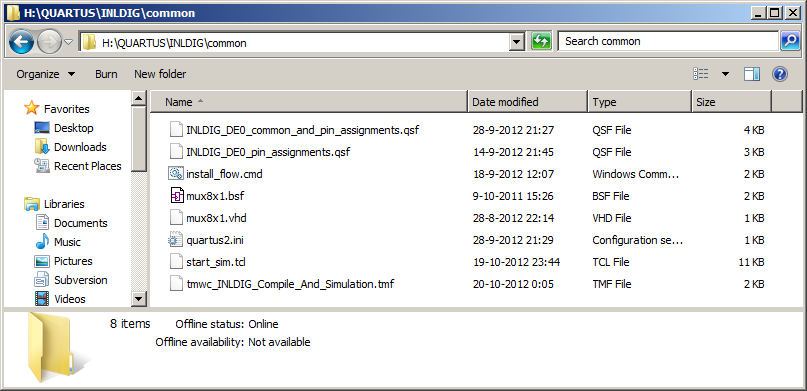
\includegraphics[scale=\tutpicscale]{008commonmap}
\caption{De inhoud van de map \lstinline|common|.}
\label{fig:008commonmap}
\end{figure}
\item Dubbelklik op het bestand \lstinline|install_flow.cmd|. Er wordt een
      scherm gestart met als uitvoer 
\begin{lstlisting}[numbers=none,belowskip=-3.5ex]
Installing INLDIG Flow... 
 1 file(s) copied. 
 1 file(s) copied. 
Press any key to continue . . . 
\end{lstlisting}
\item Druk op een toets om het scherm te sluiten. Noot: als je iets anders
ziet dan hierboven, raadpleeg de docent. 
\end{enumerate}

De flow is nu ge\"{\i}nstalleerd. We kunnen beginnen met invoeren van
de schakeling.
 
Noot: het is ook mogelijk om de bestanden handmatig in een andere map te
installeren, zie de bijlagen~\ref{chap:inldigflowonderlinux} en
\ref{chap:inldigflowonderwindows}. 


\section{Project en naamgeving}
\label{sec:projectennaamgeving}
Een project bestaat uit niets anders dan een verzameling bestanden. De
belangrijkste bestanden hebben de volgende extensies: 

\begin{table}[H]
\centering
\caption{Betekenis bestandsnaamextensies.}
\label{tab:bestandsnaamextensies}
% \usepackage{array} is required
\begin{tabular}{|>{\centering\arraybackslash}p{1.5cm}|p{5cm}|p{8cm}|}
\hline 
Extensie & Volledige naam & Betekenis  \\ \hline 
\naam{.qpf} & Quartus Project File  & Projectbestand met naam en algemene
                                      informatie \\ \hline 
\naam{.qsf} & Quartus Settings File & Instellingen bij een bepaalde \textsl{revisie},
                                      meestal is er maar \'{e}\'{e}n revisie \\ \hline 
\naam{.bdf} & Block Design File     & Schema-bestand, zoals poorten, en componenten
                                      waardoor hi\"{e}rachi\"{e}en mogelijk zijn. \\ \hline 
\naam{.bsf} & Block Schematic File  & Een component (``poort'') gemaakt van een
                                      bdf-bestand of vhd-bestand \\ \hline 
\naam{.do}  & ModelSim Command File & Bestand met commando's voor de simulator \\ \hline 
\naam{.vhd} & VHDL File             & Bestand met VHDL-code \\ \hline 
\naam{.v}   & Verilog File          & Bestand met Verilog-code, wordt tijdens
                                      het practicum niet gebruikt \\ \hline 
\naam{.sof} & SRAM Object File      & Bestand met ``code'' voor de FPGA,
                                      informatie die in de FPGA geladen moet
                                      worden \\ \hline 
\end{tabular} 
\end{table}

Quartus maakt in het simulatie- en synthesetraject nog veel meer bestanden met
extensies aan, die zijn niet van belang. ModelSim-testbenches beginnen met
\lstinline|tb_|.

\fpf{%
Een project kan automatisch in Quartus worden geopend door de dubbelklikken
op het betreffende .qpf-bestand.\\[1ex]
Niet op een .bdf-bestand dubbelklikken, want dan is er geen projectomgeving\\
beschikbaar en kan er niet gesimuleerd of gesynthetiseerd worden.\\[1ex]
Gebruik geen spaties, leestekens of ``vreemde'' tekens in bestandsnamen en
mapnamen!\\[1ex]
Gebruik geen minteken in bestandsnamen, underscores zijn wel toegestaan.}


\section{Project Tutorial starten}
\label{sec:projecttutorialstarten}
We starten Quartus op via Explorer. Navigeer naar
\lstinline|H:\QUARTUS\INLDIG\tutorial| en dubbelklik op het bestand
\lstinline|tutorial.qpf|. Zie figuur~\ref{fig:010tutorialmap}.

\begin{figure}[H]
\centering
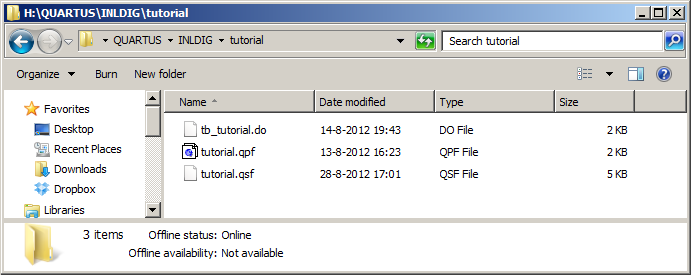
\includegraphics[scale=\tutpicscale]{010tutorialmap}
\caption{Inhoud van de map \lstinline|tutorial|.}
\label{fig:010tutorialmap}
\end{figure}

Na het opstarten \textsl{kan} figuur~\ref{fig:011infoscreen} verschijnen. Via
deze \texttt{Getting Started} kan je snel een project aanmaken of openen. We
slaan dit scherm over. Klik hiervoor op het kruisje rechtsboven.

\begin{figure}[H]
\centering
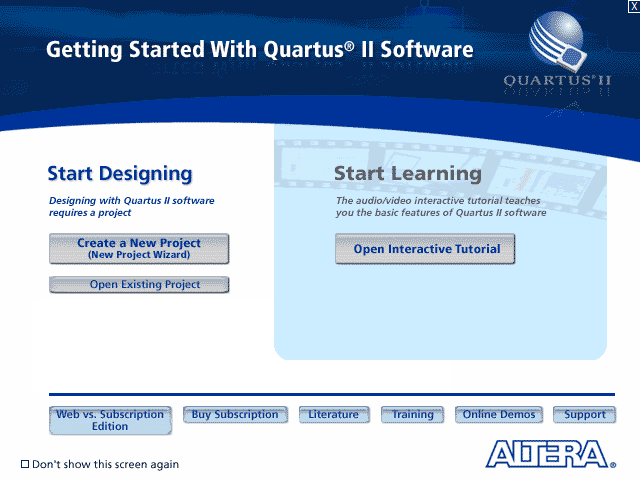
\includegraphics[scale=\tutpicscale]{011infoscreen.png}
\caption{Quartus II opstartscherm}
\label{fig:011infoscreen}
\end{figure}

De \textsl{Project Manager} wordt gestart
(figuur~\ref{fig:012quartusstartupscreen}).
De grootte en indeling van het scherm kan iets afwijken van de figuur. Probeer
dit aan te passen volgens de figuur. 

\begin{figure}[H]
\centering
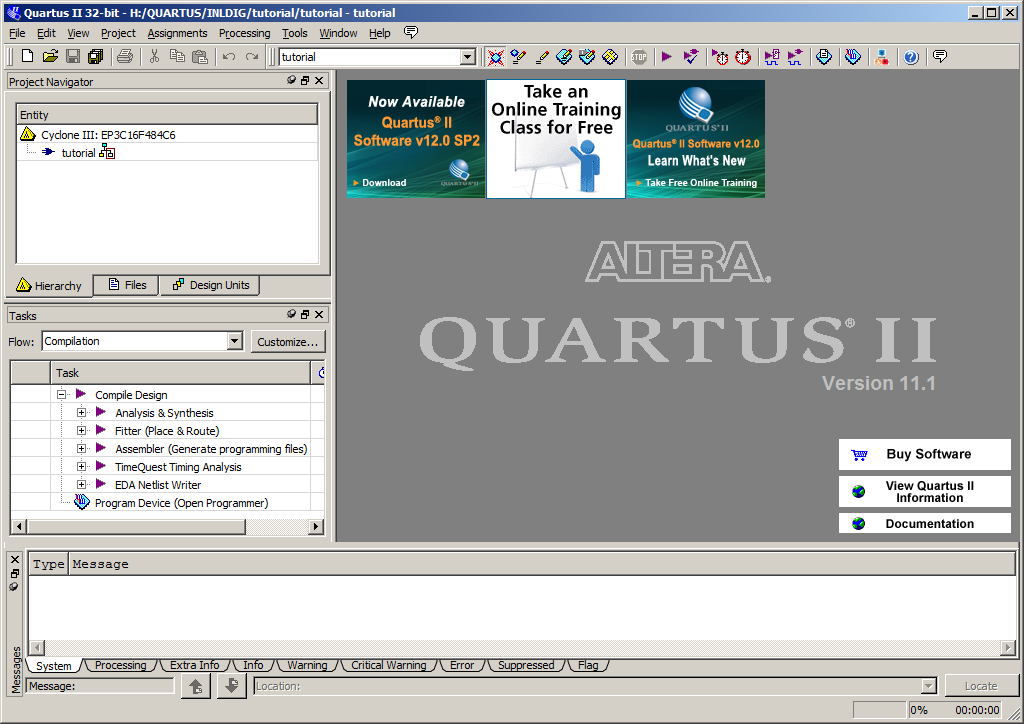
\includegraphics[scale=\tutpicscale]{012quartusstartupscreen}
\caption{Openingsscherm Project Manager}
\label{fig:012quartusstartupscreen}
\end{figure}

Indien van toepassing wordt het laatst geopende project geopend. De
\textsl{Project Manager} bestaat uit menu's, knoppenbalk en vier vensters.
Linksboven is de \textsl{Project Navigator}. Hierin worden alle (broncode-)%
bestanden en de onderlinge afhankelijkheden zichtbaar gemaakt, zoals
hi\"{e}rarchie\"{e}n en testbenches. Daaronder is de \textsl{Tasks}-venster.
Hierin worden de mogelijke taken bij een geselecteerd bestand weergegeven,
zoals synthetiseren of implementeren. Rechts is het \textsl{edit}-venster
waar bestanden bewerkt en bekeken kunnen worden. Onderaan is het
\textsl{Message}-venster waar uitvoer van de diverse opdrachten wordt
afgedrukt.

Voor de juiste werking moet eerst de \textsl{flow} worden ingesteld. In het
venster \naam{Tasks} kan je bij het onderdeel \naam{Flow} kiezen voor een
flow. Kies hier de flow \naam{INLDIG Compile And Simulation}.
Zie figuur~\ref{fig:013chooseinldigflow}.

\begin{figure}[H]
\centering
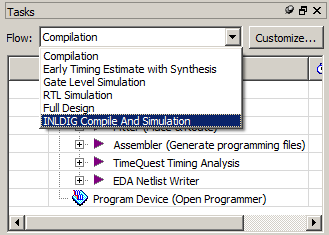
\includegraphics[scale=\tutpicscale]{013chooseinldigflow}
\caption{Selecteren van de INLDIG-flow.}
\label{fig:013chooseinldigflow}
\end{figure}

Kies in het venster \textsl{Project Navigator} voor het tabblad \naam{Files}.
Hier zie je een overzicht van de bestanden die tot het project behoren. Het
project bestaat uit slechts \'{e}\'{e}n bestand genaamd
\lstinline|tb_tutorial.do|. Zie figuur~\ref{fig:014selectfilestab}.

\begin{figure}[H]
\centering
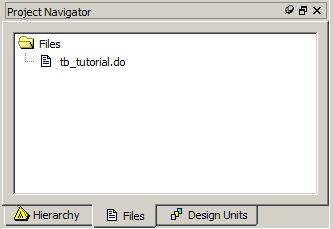
\includegraphics[scale=\tutpicscale]{014selectfilestab}
\caption{Het \lstinline|Files|-tabblad.}
\label{fig:014selectfilestab}
\end{figure}


\section{Aanmaken schemabestand}
\label{sec:aanmakenschemabestand}
We gaan nu het eerste schema invoeren. Dit schema gaat later gebruikt worden
als ``poort'' in een ander schema. 
 
Als eerste zullen we een schemabestand in het project aanmaken. Klik in de
Project Manager op \menu{File\pijl{}New} (figuur~\ref{fig:015createnewfile}).
Als alternatief kan de toetscombinatie \knop{Ctrl+N} gebruikt worden. 

\begin{figure}[H]
\centering
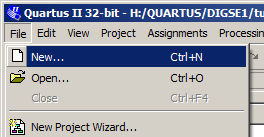
\includegraphics[scale=\tutpicscale]{015createnewfile}
\caption{Aanmaken nieuw bestand.}
\label{fig:015createnewfile}
\end{figure}

Nu verschijnt er een scherm waarin je het type van het nieuwe bestand kan
kiezen (figuur~\ref{fig:016selectblockschematic}). Kies voor
\naam{Block Diagram/Schematic File}.
 
\begin{figure}[H]
\centering
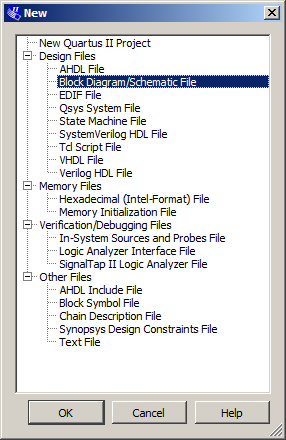
\includegraphics[scale=\tutpicscale]{016selectblockschematic}
\caption{Keuze bestandstype.}
\label{fig:016selectblockschematic}
\end{figure}

De Project Manager opent nu een leeg bestand. Dit is te zien in
figuur~\ref{fig:018screenwithopenblockfile}. Merk op dat het bestand de
tijdelijk naam \naam{Block1.bdf} heeft.
Het sterretje achter de naam geeft aan dat het bestand gewijzigd en nog niet opgeslagen is.
Bij het opslaan van het bestand kan
alsnog een andere naam worden ingevoerd.

\begin{figure}[H]
\centering
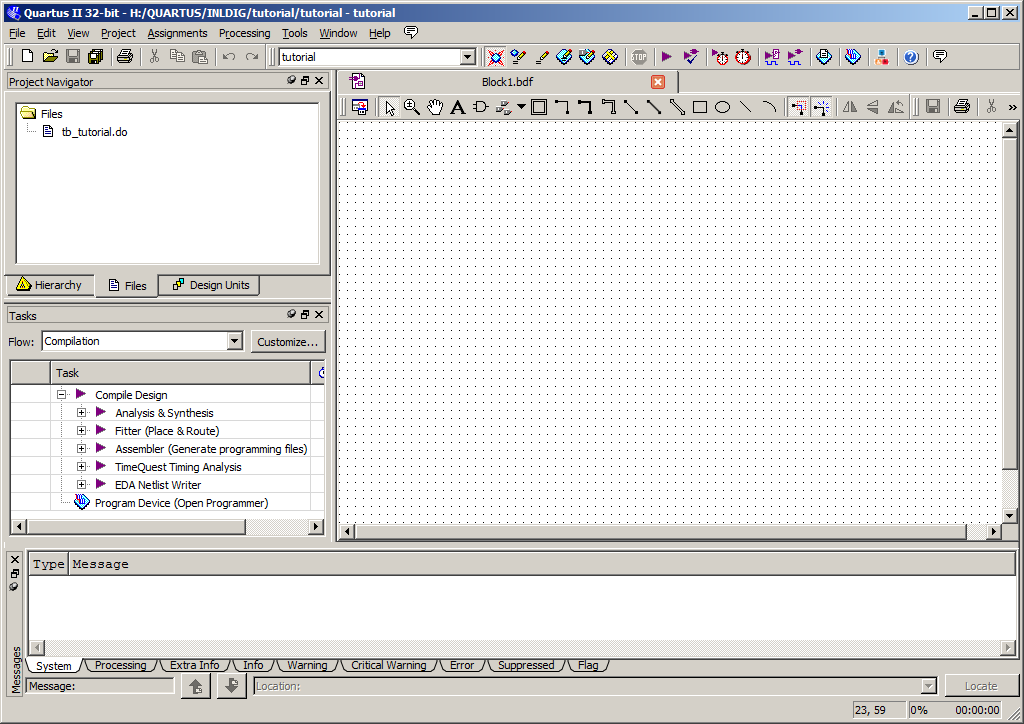
\includegraphics[scale=\tutpicscale]{018screenwithopenblockfile}
\caption{Overzicht Quartus IDE na aanmaken nieuw BDF-bestand.}
\label{fig:018screenwithopenblockfile}
\end{figure}

Bovenaan het edit-venster staat een rij knoppen. De twee belangrijkste zijn
de poortinvoerknop (\naam{symbol tool}, ziet eruit als een AND-poort) en
de pin-invoerknop (\naam{pin tool}).
Zie figuur~\ref{fig:021schematictoolbarcooked}. 

\begin{figure}[H]
\centering
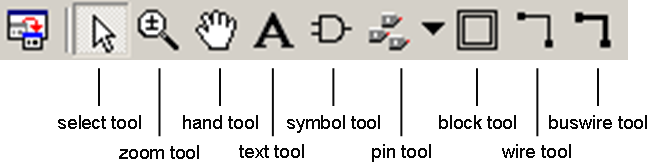
\includegraphics[scale=\tutpicscale]{021schematictoolbarcooked}
\caption{Overzicht van de knoppen.}
\label{fig:021schematictoolbarcooked}
\end{figure}

Klik nu op het AND-poortje. Er wordt een dialoogvenster geopend.
Zie figuur~\ref{fig:022symbolselection}.

\begin{figure}[H]
\centering
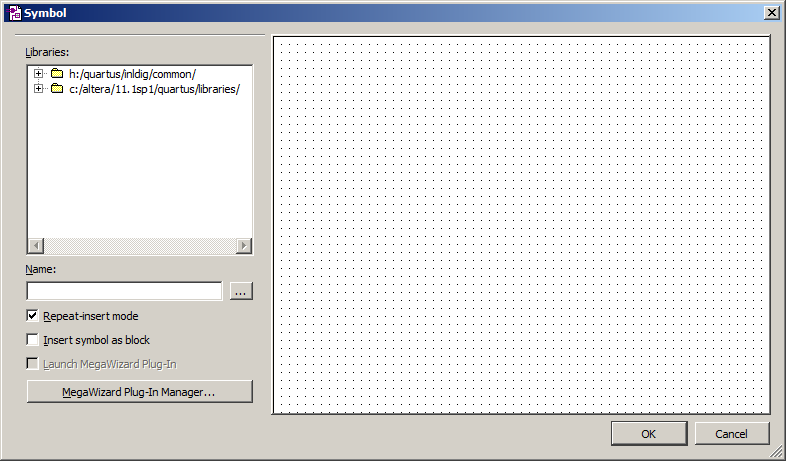
\includegraphics[scale=\tutpicscale]{022symbolselection}
\caption{Selectie component.}
\label{fig:022symbolselection}
\end{figure}

Linksboven staan de \textsl{libraries} (bibliotheken) vermeld. Hierin zijn de
poorten opgenomen die we gaan gebruiken.

Noot: als de de eerste regel in figuur~\ref{fig:022symbolselection} niet
ziet, dan heb je bij het installeren van de projectomgeving niet de
juiste mappenstructuur aangemaakt. Zorg ervoor dat de mappen \naam{common}
en \naam{tutorial} in de map \lstinline|H:\QUARTUS\INLDIG\| geplaatst zijn.

Open nu de tweede library tot op het niveau van \naam{logic} en selecteer
de AND2-poort. Zie figuur~\ref{fig:023withandport}.

\begin{figure}[H]
\centering
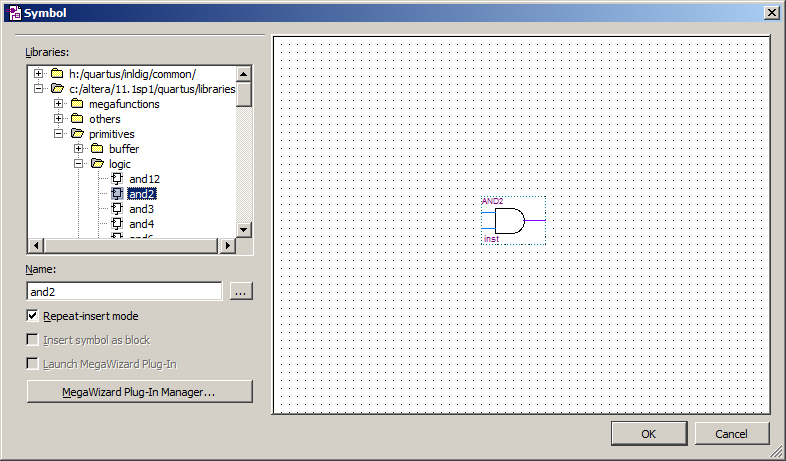
\includegraphics[scale=\tutpicscale]{023withandport}
\caption{Selectie AND2-poort.}
\label{fig:023withandport}
\end{figure}

Klik op \knop{OK}. De AND2-poort ``hangt'' nu aan de cursor. Plaats de poort
ergens in het midden van het edit-venster. 

Noot: na het plaatsen ``hangt'' er opnieuw een AND2-poort aan de cursor. Je
kan er dus nog \'{e}\'{e}n plaatsen. Dit wordt de \textsl{Repeat-insert Mode}
genoemd. Druk op de \knop{ESC}-toets om dit af te breken.

Noot: in figuur~\ref{fig:023withandport} zie je een niveau genaamd
\naam{others}. Gebruik \textbf{geen} poorten uit dit deel van de bibliotheek.
 
Voeg nu op gelijke wijze een NOT-poort in. Deze poort zit iets lager in
dezelfde kolom. 
 
Nu moeten de ingangs- en uitgangspoorten nog worden geplaatst. Dit kan op twee
manieren: via de \naam{symbol tool} (maar dan onder het niveau \naam{pin})
of via de pin tool. Klik hiervoor op het driehoekje van pin tool
pictogram en selecteer \naam{Input}. Zie figuur~\ref{fig:025selectinput}.

\begin{figure}[H]
\centering
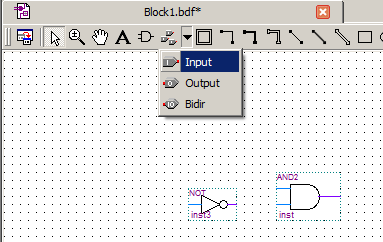
\includegraphics[scale=\tutpicscale]{025selectinput}
\caption{Selectie input-poort.}
\label{fig:025selectinput}
\end{figure}

Plaats nu twee input-pinnen in het edit-venster. Selecteer via de pin tool nu
\naam{Output} en plaats een output-pin.
Zie figuur~\ref{fig:026schematicnowires}.

\begin{figure}[H]
\centering
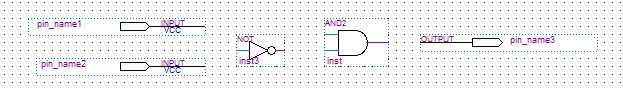
\includegraphics[scale=\tutpicscale]{026schematicnowires}
\caption{Alle geplaatste componenten.}
\label{fig:026schematicnowires}
\end{figure}

Nu moeten de diverse pinnen en poorten aan elkaar verbonden worden. Dat gaat
vrij makkelijk. Plaats de cursor boven het eindpunt van de bovenste input-pin.
Druk op de linker muisknop en houdt deze ingedrukt. Sleep nu naar \textsl{vlak
voor} de bovenste ingang van de AND2-poort en laat de muisknop los. Er
verschijnt nu een blauwe lijn. Maak nu een kleine lijn haaks naar beneden en 
vervolgens een lijn naar AND2-poort. Klik dan even in het edit-veld zodat de
blauwe lijn gedeselecteerd wordt. De lijn wordt nu paars. Verbind vervolgens
ook de andere componenten zoals aangegeven in figuur~\ref{fig:027withwires}.

\begin{figure}[H]
\centering
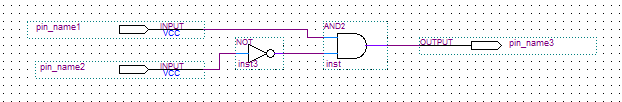
\includegraphics[scale=\tutpicscale]{027withwires}
\caption{Alle geplaatste componenten met verbindingen.}
\label{fig:027withwires}
\end{figure}

Als laatste stap moeten de ingangen en uitgangen nog een nieuwe naam krijgen.
Dubbelklik precies op de naam \naam{pin\_name1}. De naam wordt nu
geselecteerd. Verander dit in \naam{x} (kleine letter). Vervang nu ook
\naam{pin\_name2} door \naam{y} en \naam{pin\_name3} door \naam{f}. Het geheel
is te zien in figuur~\ref{fig:028withpinnames}. 

\begin{figure}[H]
\centering
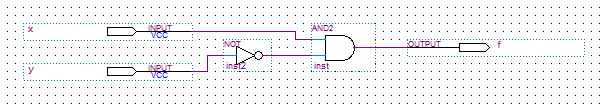
\includegraphics[scale=\tutpicscale]{028withpinnames}
\caption{Schema met nieuwe pinnamen.}
\label{fig:028withpinnames}
\end{figure}

Nu het schema is ingevoerd, moet het bestand opgeslagen worden. Klik in de
Project Manager op \menu{File\pijl{}Save} (zie figuur~\ref{fig:029savefile}).
 
\begin{figure}[H]
\centering
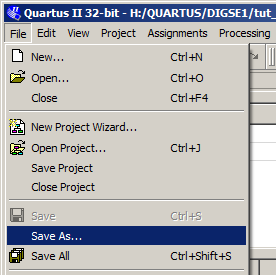
\includegraphics[scale=\tutpicscale]{029savefile}
\caption{Bestand opslaan.}
\label{fig:029savefile}
\end{figure}

Er wordt een scherm geopend waarin de juiste map en de bestandsnaam ingevuld
kunnen worden. Zie figuur~\ref{fig:030savefileas}. Er wordt een bestandsnaam
voorgesteld, wijzig dit in \naam{inhibit.bdf}. Let op het vinkje bij
\naam{Add file to current project}.
 
\begin{figure}[H]
\centering
%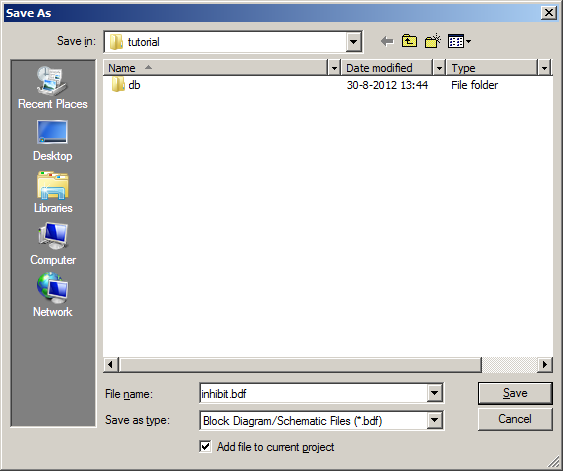
\includegraphics[scale=\tutpicscale]{030savefileas}
\begin{overpic}[scale=\tutpicscale,unit=1mm]{030savefileas}
\linethickness{1pt}
\color{red}\put(32.5,12.3){\oval(20,5)}
\end{overpic}
\caption{Opgeven bestandsnaam BDF-bestand.}
\label{fig:030savefileas}
\end{figure}

\textbf{Noot:} je mag geen spaties, leestekens of ``vreemde'' tekens in de
bestandsnaam opnemen! \\
\textbf{Noot:} let goed op de map waarin het bestand opgeslagen wordt. Quartus
wil nog wel eens de map van een eerder geopend project presenteren. \\
\textbf{Noot:} bestandsnaam \textsl{niet} met een cijfer beginnen!

Het bestand is nu terug te vinden in de Project Navigator onder het tabblad
\naam{Files}. Zie figuur~\ref{fig:031fileinproject}.
 
\begin{figure}[H]
\centering
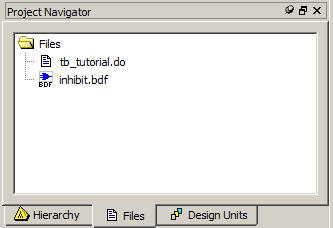
\includegraphics[scale=\tutpicscale]{031fileinproject}
\caption{Het opgeslagen bestand staat in de lijst van bestanden.}
\label{fig:031fileinproject}
\end{figure}


\section{Aanmaken van symbool van het huidige bestand}
\label{sec:aanmakenvansymboolvanhethuidigebestand}
We gaan het schema dat net is opgeslagen in een ander schema gebruiken.
Hiervoor moet eerst een \textsl{symbol} worden aangemaakt van het schema.
Dit symbol komt dan terug in de \textsl{library}. 
 
Open het bestand \lstinline|inhibit.bdf| of, als het bestand al geopend is,
selecteer in het edit-venster het tabblad van het bestand. Selecteer via het
menu \menu{File\pijl{}Create/Update\pijl{}Create Symbol Files for Current File}.
Zie figuur~\ref{fig:033createsymbolfiles}.

\begin{figure}[H]
\centering
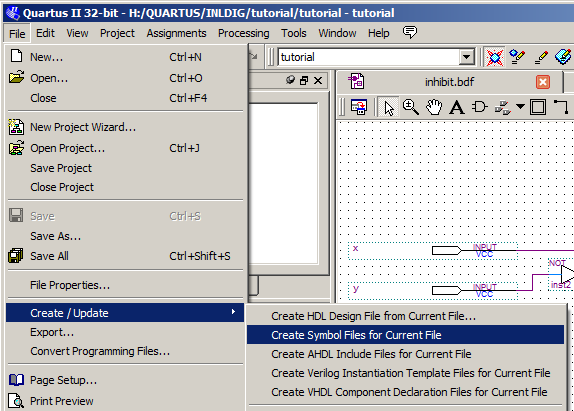
\includegraphics[scale=\tutpicscale]{033createsymbolfiles}
\caption{Aanmaken nieuw symbool.}
\label{fig:033createsymbolfiles}
\end{figure}

Er wordt een dialoogvenster geopend waarin een bestandsnaam kan worden
ingevoerd. De voorgestelde naam \naam{inhibit.bsf} is goed. Klik op \knop{OK}
om het bestand op te slaan. Zie figuur~\ref{fig:034savefileas}.

\begin{figure}[H]
\centering
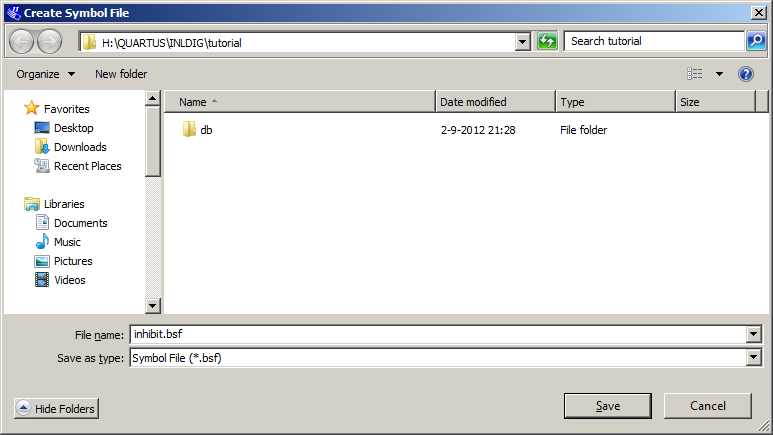
\includegraphics[scale=\tutpicscale]{034savefileas}
\caption{Bestandsnaam nieuw symbool.}
\label{fig:034savefileas}
\end{figure}

Quartus komt met de melding dat het bestand is aangemaakt.
Zie figuur~\ref{fig:035bsffilecreated}.

\begin{figure}[H]
\centering
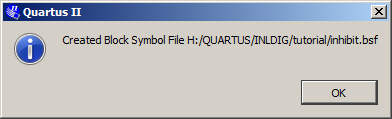
\includegraphics[scale=\tutpicscale]{035bsffilecreated}
\caption{Het bestand is opgeslagen.}
\label{fig:035bsffilecreated}
\end{figure}


\section{Aanmaken van een tweede schemabestand}
\label{sec:aanmakenvaneentweedeschemabestand}
We maken nu op dezelfde wijze een nieuw schemabestand aan (zie
figuren~\ref{fig:015createnewfile} en \ref{fig:016selectblockschematic}).
Plaats daarin de net aangemaakt ``poort''. Deze kan je vinden onder onder
de library \naam{Project}. Zie figuur~\ref{fig:037selectinhibit}.
 
\begin{figure}[H]
\centering
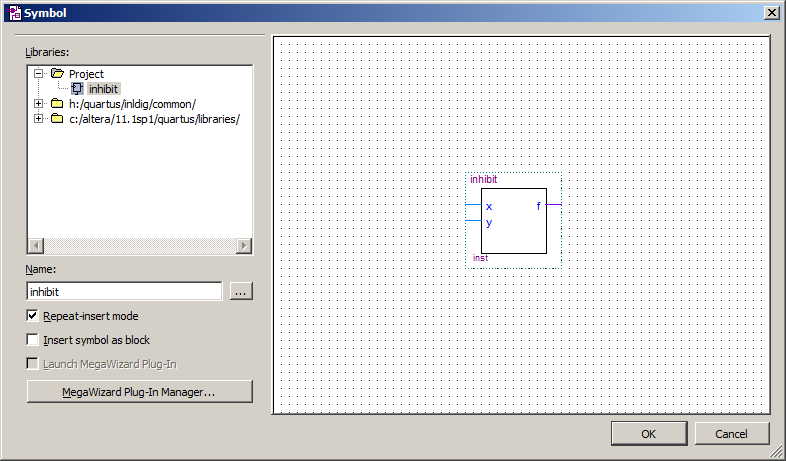
\includegraphics[scale=\tutpicscale]{037selectinhibit}
\caption{Selectie nieuwe component.}
\label{fig:037selectinhibit}
\end{figure}

Plaats deze ``poort'' ergens in het edit-venster. Maak het schema verder af
zoals in aangegeven in figuur~\ref{fig:038schematictoplevel}. Let goed op de
poorten; er moeten een OR2- en een XOR-poort geplaatst worden. 
 
\begin{figure}[H]
\centering
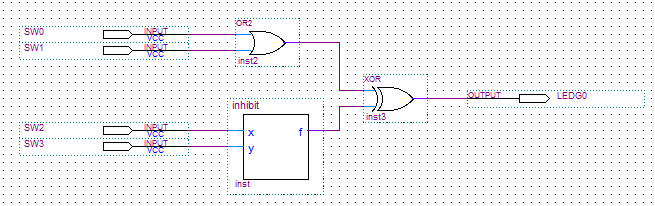
\includegraphics[scale=\tutpicscale]{038schematictoplevel}
\caption{Het bestand is opgeslagen.}
\label{fig:038schematictoplevel}
\end{figure}

Let goed op de namen van de ingangen en uitgang (hoofdletters!). 
 
Sla het bestand op onder de naam \naam{tutorial.bdf}. De naam van het bestand
komt nu in de lijst van bestanden bij de Project Navigator.


\section{Eerste synthese}
\label{sec:eerstesynthese}
Om te controleren of het schema \textsl{syntactisch correct} is en er hardware
voor kan worden gegenereerd zullen we de synthesizer starten. Klik in de Project
Manager op \menu{Processing\pijl{}Start\pijl{}Start Analysis \& Synthesis} of
gebruik de sneltoetscombinatie \menu{Ctrl+K}. Zie
figuur~\ref{fig:039startanalysis}.
 
\begin{figure}[H]
\centering
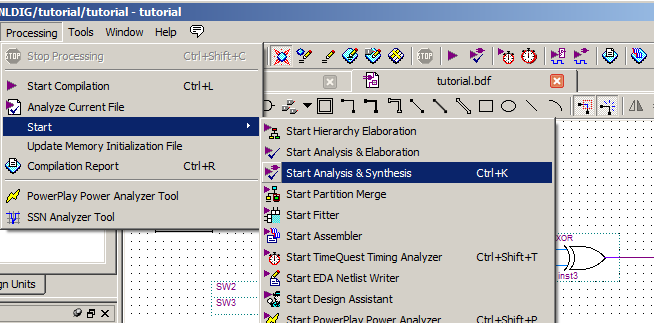
\includegraphics[scale=\tutpicscale]{039startanalysis}
\caption{Starten Analysis \& Synthesis vanuit het menu.}
\label{fig:039startanalysis}
\end{figure}

Als deze stap gelukt is zie je onder \naam{Tasks} een paar vinkjes verschijnen
en je krijgt een melding (figuur~\ref{fig:040analysissynthesissuccessful}).
Klik op \knop{OK} om verder te gaan.
 
\begin{figure}[H]
\centering
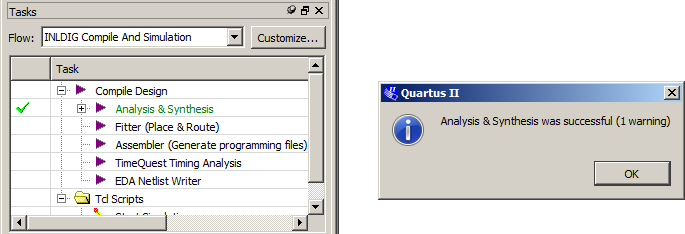
\includegraphics[scale=\tutpicscale]{040analysissynthesissuccessful}
\caption{De analyse is gelukt.}
\label{fig:040analysissynthesissuccessful}
\end{figure}

Mocht je een fout hebben gemaakt, bijvoorbeeld twee ingangen aan elkaar
verbonden, dan zal de synthesizer dat melden, zie
figuur~\ref{fig:041notsuccesful}.
Merk op dat de fout in de schakeling \naam{inhibit} zit.

\begin{figure}[H]
\centering
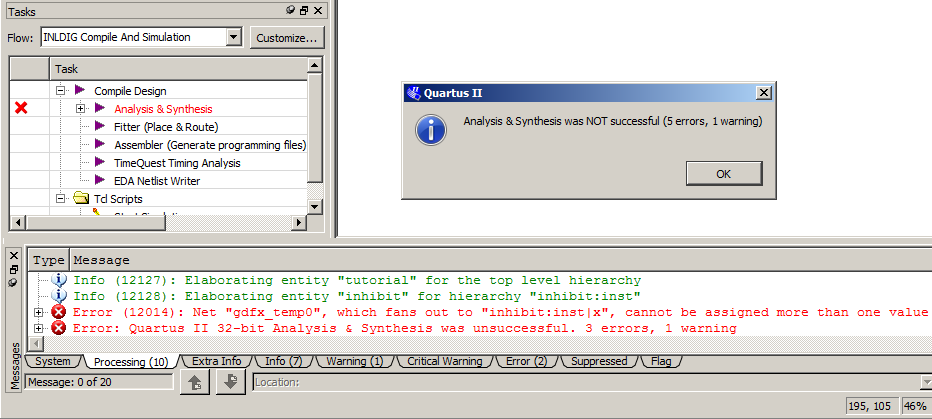
\includegraphics[scale=\tutpicscale]{041notsuccesful}
\caption{De analyse is mislukt.}
\label{fig:041notsuccesful}
\end{figure}

\section{Simulatie poortschakeling}
\label{sec:simulatiepoortschakeling}
Nu de schema's ingevoerd zijn, moet het geheel gesimuleerd te worden. Dit
droogzwemmen is bedoeld om te kunnen verifi\"{e}ren of de schakeling, en dus
de schema's, werkt volgens de specificaties. Het Quartus II pakket gebruikt
hiervoor de externe simulator ModelSim van firma Mentor Graphics. We gebruiken
de simulator om aan te tonen dat onze schakeling functioneel correct is. Het
kan namelijk best zijn dat de schakeling gesynthetiseerd kan worden, maar dat
de schakeling niet doet wat het zou moeten doen. Bij deze simulatie worden
geen vertragingstijden meegenomen.
 
Voor simulatie is een zogenaamd scriptbestand nodig. Hierin staan opdrachten
voor de simulator. Je kan deze opdrachten ook interactief op een commandoregel
invoeren, maar vaak wil je de simulatie een paar keer opnieuw draaien. Dan is
het steeds invoeren van de (zelfde reeks) commando's een tijdrovende zaak. 
In het scriptbestand staat een aantal opdrachten die de simulator gebruikt om
de ingangen mee aan te sturen. Dit zijn de zogenaamde \textsl{stimuli}. De
simulator gebruikt deze waarden om de schakeling door te rekenen. 
 
Noot: de commando's staan het het bestand \naam{tb\_tutorial.do} dat al is
aangemaakt. Je kan de inhoud van het bestand bekijken, maar laat de inhoud
ongewijzigd anders kan de simulatie mislukken. 
 
Dubbelklik in het Tasks-venster op \naam{Start Simlation}, zie
figuur~\ref{fig:043startsimulation}.

\begin{figure}[H]
\centering
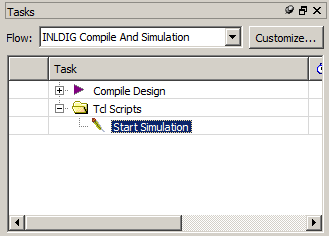
\includegraphics[scale=\tutpicscale]{043startsimulation}
\caption{Starten van de simulatie.}
\label{fig:043startsimulation}
\end{figure}

Tijdens het starten van ModelSim wordt een \textsl{splashscreen} getoond.
De simulator wordt gestart (dit kost enige tijd) en er worden vijf vensters
geopend (zie figuur~\ref{fig:044modelsimstarted}). 

\begin{figure}[H]
\centering
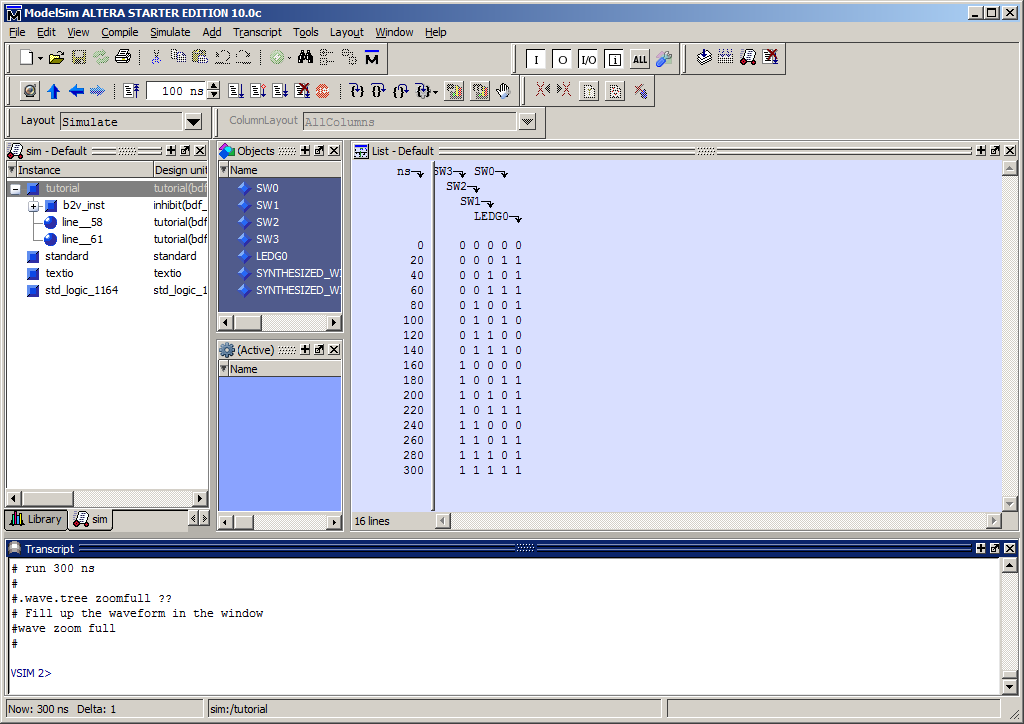
\includegraphics[scale=\tutpicscale]{044modelsimstarted}
\caption{Het resultaat van de simulatie.}
\label{fig:044modelsimstarted}
\end{figure}

Onderaan is de \textsl{Transcript Window}. Hier kan je ook losse commando's
geven (voor gevorderden). Rechts is de \textsl{List Window}. De overige drie
zijn op dit moment niet van belang. 
 
In de List Window wordt de uitkomst van de simulatie weergegeven. Je ziet een
aantal rijen. Een rij wordt voorafgegaan aan een getal (dat is een
simulatietijd) en daarna vijf nullen of enen. De eerste vier stellen de
waarden voor van de vier ingangen \naam{SW3} t/m \naam{SW0}, de laatste de
waarde van de uitgang \naam{LEDG0}. Deze namen komen overeen met de schakelaars
en leds van het ontwikkelbordje. Zie hoofdstuk~\ref{chap:ontwikkelbordje}.

Je kan het commando-script nogmaals uitvoeren door in de transcript window
op de $\uparrow$-toets te drukken. Het laatst ingevoerde commando verschijnt
dan. Druk op de \knop{enter}-toets om dat commando uit te voeren. Zie
figuur~\ref{fig:045transcriptwindow}.

\begin{figure}[H]
\centering
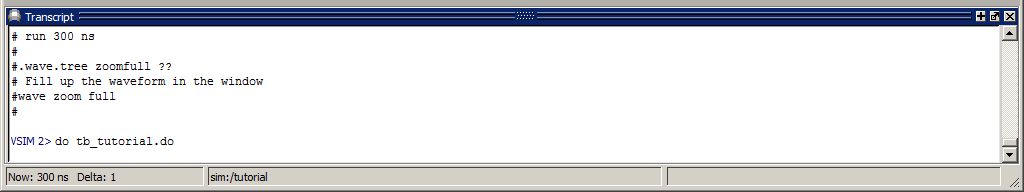
\includegraphics[scale=\tutpicscale]{045transcriptwindow}
\caption{Het transcript-window.}
\label{fig:045transcriptwindow}
\end{figure}

De simulatie is nu ten einde. Sluit de simulator af via het menu
\menu{File\pijl{}Quit}. Er wordt een dialoogvenster geopend, zie
figuur~\ref{fig:046wantoquit}. Klik op \knop{Yes}.

\begin{figure}[H]
\centering
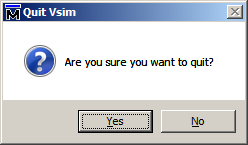
\includegraphics[scale=\tutpicscale]{046wantoquit}
\caption{ModelSim afsluiten.}
\label{fig:046wantoquit}
\end{figure}


\section{Compilatie}
\label{sec:compilatie}
Nu de simulatie uitgevoerd is, wordt de schakeling gecompileerd. Compileren
valt uiteen in twee delen: synthese en implementatie. Synthese houdt in dat de
schakeling wordt vertaald met als resultaat een netlist; een beschrijving van
de digitale logica in primitieven. Denk hierbij aan poorten, flipflops, LUTs
(LookUp Table, ROM) of speciale voorzieningen zoals Phase Locked Loops of
klokbuffers. Deze primitieven zijn voor elk configureerbaar type weer anders. 
Implementatie houdt in dat de primitieven worden \textsl{gemapped} op de LE's.

Start de compilatie via de menuoptie \menu{Processing\pijl{}Start Compilation}
of gebruik de sneltoetscombinatie \knop{Ctrl+L}.
Zie figuur~\ref{fig:050startcompilation}.

\begin{figure}[H]
\centering
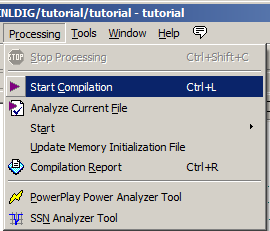
\includegraphics[scale=\tutpicscale]{050startcompilation}
\caption{Starten van de compilatie.}
\label{fig:050startcompilation}
\end{figure}

De compilatie wordt nu gestart. Dat kan afhankelijk van het ontwerp enige tijd
duren. Je kan de voortgang in het \menu{Tasks}-venster. Als de compilatie geen
fouten oplevert krijg je een melding zoals in
figuur~\ref{fig:051compilecomplete}. In het algemeen zijn de waarschuwingen niet
problematisch, maar kijk de meldigen toch even na.
 
\begin{figure}[H]
\centering
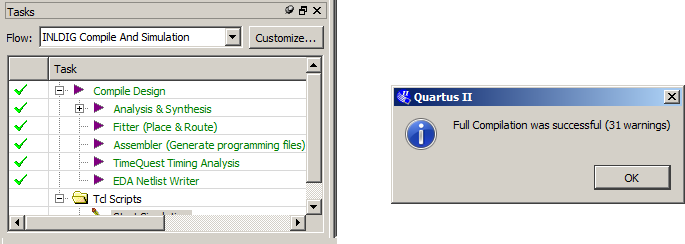
\includegraphics[scale=\tutpicscale]{051compilecomplete}
\caption{De compilatie is gelukt.}
\label{fig:051compilecomplete}
\end{figure}

Je krijgt na compilatie een rapport met alle verrichte werkzaamheden. Een
interessant onderdeel hiervan is het aantal gebruikte
\textsl{Logic Elements}. Hieraan kan je zien hoe groot je ontwerp is.
Zie figuur~\ref{fig:052flowsummary}.

\begin{figure}[H]
\centering
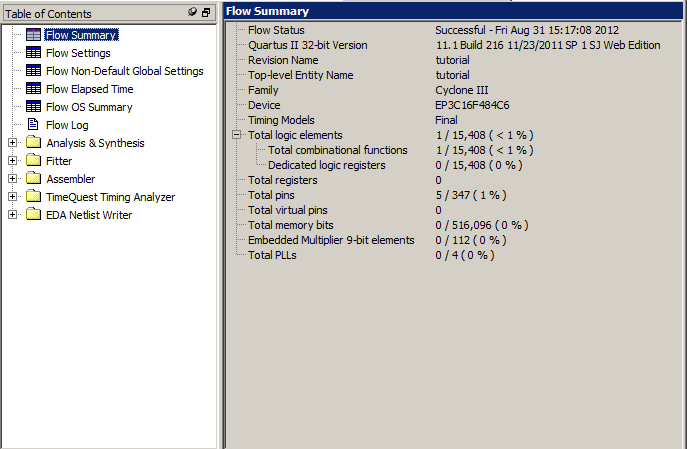
\includegraphics[scale=\tutpicscale]{052flowsummary}
\caption{Overzicht van het resultaat van de compilatie.}
\label{fig:052flowsummary}
\end{figure}

%De programmatuur is ontwikkeld door Quartus. Er zijn ook andere \textsl{tool chains} verkrijgbaar die 
%VHDL-code met hoog abstractieniveau kunnen compileren. Die van Quartus kan dat niet; alleen 
%RTL-beschrijvingen (Register Transfer Level) zijn mogelijk. We zullen ons hier aan houden.

\section{Configureren van de Cyclone III}
\label{sec:configureren}

De compilatiestap is nu afgerond. We gaan verder met het configureren
van de Cyclone III. Dat doen we gaan door het configuratiebestand in
deze component te laden. Dat gaat volgens het JTAG-protocol. Dit protocol
stelt de gebruiker in staat een hele keten van componenten te configureren.
Dit is erg handig omdat je zo updates in de componenten kan laden, ook al
zijn ze al op een print gemonteerd.

Zorg ervoor dat de USB-kabel juist is aangesloten en het ontwikkelbord is
aangezet. Als je dit  vergeet, zal de software een foutmelding geven.

\fpf{Raadpleeg de docent voordat je de apparatuur aansluit en aanzet!}

Selecteer in de Project Manager de menuoptie \menu{Tools\pijl{}Programmer}
(figuur~\ref{fig:054startprogrammer}).

\begin{figure}[H]
\centering
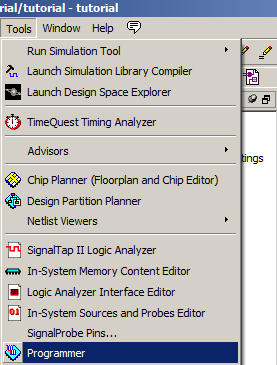
\includegraphics[scale=\tutpicscale]{054startprogrammer}
\caption{Starten van de programmer.}
\label{fig:054startprogrammer}
\end{figure}

De programmer wordt gestart (figuur~\ref{fig:056programmer}).

\begin{figure}[H]
\centering
%\includegraphics[scale=\tutpicscale]{097programmerwithfileloaded.png}
\begin{overpic}[scale=\tutpicscale,unit=1mm]{056programmer}
\linethickness{1pt}
\color{red}\put(30,66.2){\oval(35,5)}
\end{overpic}
\caption{Overzicht van de Programmer IDE.}
\label{fig:056programmer}
\end{figure}

Je kan zien of de programmer het ontwikkelbord heeft gevonden als in het
veld naast \naam{Hardware Setup} de regel \naam{USB-Blaster [USB-0]} 
staat. %Zo niet, klik dan op \menu{Hardware Setup} en selecteer de Blaster.

Als in het veld naast \naam{Hardware Setup} de opmerking \naam{No Hardware}
staat, klik dan op de knop \menu{Hardware Setup}.
\textbf{\underline{Dubbelklik}} in het geopende dialoogvenster op
\naam{USB-Blaster} in de lijst bij \naam{Available Hardware Items} en klik
daarna op de knop \menu{Close}. Zie figuur~\ref{fig:055selectusbblaster}.

Je ziet ook dat de programmer een bestand \naam{tutorial.sof} heeft
geselecteerd. Dit is het configuratiebestand dat in de Cyclone III geladen
moet worden.
 
\begin{figure}[H]
\centering
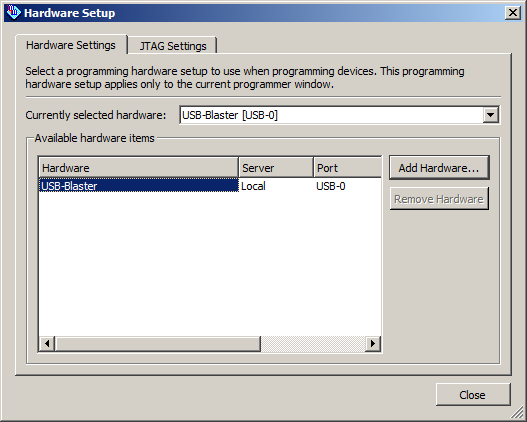
\includegraphics[scale=\tutpicscale]{055selectusbblaster}
\caption{Selecteren van de USB-Blaster download-hardware.}
\label{fig:055selectusbblaster}
\end{figure}

Druk op \knop{Start} om de Cyclone III te configureren. Daarna kan je het
ontwerp testen door middel van de schakelaars en de leds.

De tutorial is nu ten einde. Veel succes met het practicum.


\ifbetaversion

\chapter{Tips, tricks \& troubleshoot}
\label{chap:tipstrickstroubleshoot}
In dit hoofdstuk wordt een aantal veel voorkomende problemen toegelicht en hoe
je ze kunt verhelpen. Daarnaast natuurlijk de tips \& tricks.


%\section{Foutmelding Top-level undefined}
%\label{sec:fouttoplevel}
%Onderstaande foutmelding geeft aan (zie figuur~\ref{fig:220undefinedtoplevelentity})
%dat de ingestelde \textsl{top-level design entity} niet gedefinieerd is. De
%kwalificatie \textsl{top-level} slaat op de allerhoogste design entity (denk aan
%VHDL-entity) en die kan niet gevonden worden of is niet gedefinieerd.
%
%\begin{figure}[H]
%\centering
%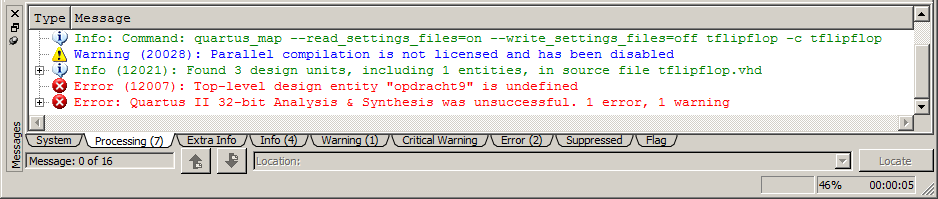
\includegraphics[scale=\tutpicscale]{220undefinedtoplevelentity.png}
%\caption{De top-level entity is niet gevonden.}
%\label{fig:220undefinedtoplevelentity}
%\end{figure}
%
%Dit gebeurt meestal omdat bij het aanmaken van een nieuw project de verkeerde
%naam is ingevuld (zie figuur~\ref{fig:025enterdirandname}). In het voorbeeld is
%de naam \naam{opdracht9} ingevuld terwijl bij de \naam{entity}-beschrijving in
%VHDL een andere naam is gebruikt. Gelukkig kan in Quartus een andere entity
%als top-level worden ingesteld. Selecteer via het menu
%\menu{Assignments\pijl{}Settings} of gebruik de sneltoets \menu{Ctrl+Shift+E}.
%Zie figuur~\ref{fig:074assignmentssettings}. Klik in het nieuw geopende dialoog
%links boven op \naam{General}.
%
%Rechts kan een ander top-level gekozen worden op op de knop met de drie puntjes
%te klikken achter het veld met \naam{Top level entity:} waarna in een klein venster
%de nieuwe naam gekozen kan worden. Klik dan op \knop{Ok}. Het kleine venster wordt
%afgesloten. Klik in de dialoog eerst op knop \knop{Apply} en daarna op knop \knop{Ok}.
%Zie figuur~\ref{fig:222selecttoplevelentity}. De dialoog wordt afgesloten.
%
%In de Program Navigator is nu de nieuwe top-level entity te vinden.
%
%\begin{figure}[H]
%\centering
%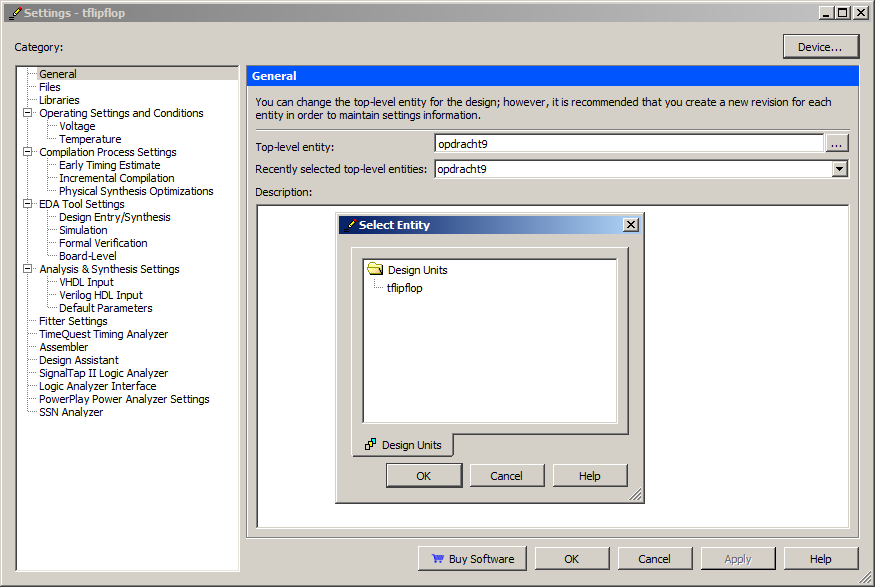
\includegraphics[scale=\tutpicscale]{222selecttoplevelentity.png}
%\caption{Selectie van top-level entity.}
%\label{fig:222selecttoplevelentity}
%\end{figure}
%


\section{Instellen pad naar ModelSim}
\label{sec:instellenmodelsimpad}
Als in Quartus het pad naar ModelSim niet correct is ingesteld, krijg je de volgende foutmelding 
(figuur~\ref{fig:210modelsimpath_121}).

\begin{figure}[H]
\centering
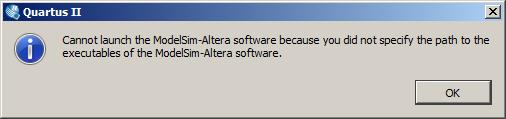
\includegraphics[scale=\tutpicscale]{210modelsimpath_121.png}
\caption{De simulator kan niet worden gestart.}
\label{fig:210modelsimpath_121}
\end{figure}

Ga als volgt te werk:

\begin{itemize}\itemsep-1pt
\item Open in de Project manager het menu \menu{Tools\pijl{}Options}
\item In het venster dat geopend wordt kies je \menu{EDA Tool Options}
\item Aan de rechterkant kan je in het veld \naam{ModelSim-Altera} het pad opgeven.
\item Voor de PC's op school is dat \lstinline|C:\altera\13.0sp1\modelsim_ase\win32aloem|
\end{itemize}

Op je eigen PC hangt dat af van het installatie-pad.
% Bij gebruik van de Web
%Edition moet je \naam{modelsim\_ae} vervangen voor \naam{modelsim\_ase}.
 Zie
figuur~\ref{fig:212modelsimpath2}.

Tip: bij gebruik van Quartus v13.1 moet je een \lstinline|\| (``backslash'')
achter de padnaam zetten.

\begin{figure}[H]
\centering
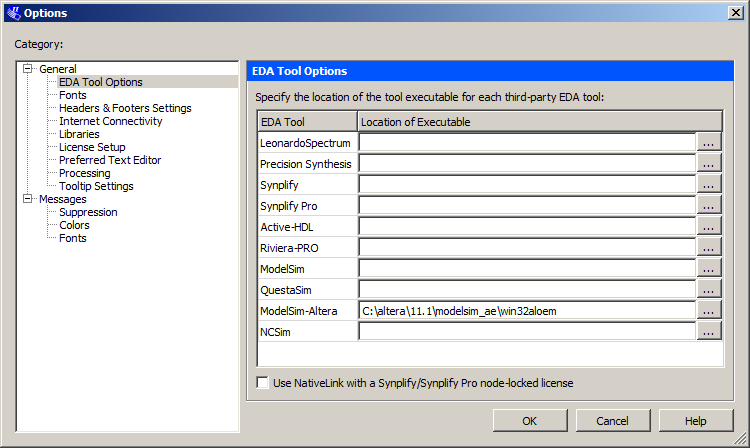
\includegraphics[scale=\tutpicscale]{212modelsimpath2.png}
\caption{Instellen van pad naar ModelSim.}
\label{fig:212modelsimpath2}
\end{figure}


\section{Smart compilation}
\label{sec:smartcompilation}
Quartus heeft de neiging om bij een compilatie-opdracht alle stappen te
doorlopen, ook als dat niet nodig is. Denk bijvoorbeeld aan het instellen van
een nieuwe top-level entity. Dan is synthese niet nodig, die is al een keer
uitgevoerd. Als een project meerdere VHDL-bestanden bevat, is het niet nodig
om alle bestanden opnieuw te synthetiseren, alleen de bestanden die aangepast
zijn.

Quartus heeft een optie die \textsl{Smart compilation} wordt genoemd en
alleen die stappen doorloopt die nodig zijn voor het eindresultaat. Open via
het menu \menu{Assignments\pijl{}Settings}. Selecteer in het gedeelte
\naam{Catagory} de optie \naam{Compilation Process Settings}. Aan de 
rechterkant verschijnen de instellingen voor compilatie. Zet een vinkje
bij de optie \naam{Use smart compilation} en sluit het venster af
door eerst op knop \knop{Apply} te drukken en daarna op knop \knop{Ok}.
Zie figuur~\ref{fig:225smartcompilation}.

\begin{figure}[H]
\centering
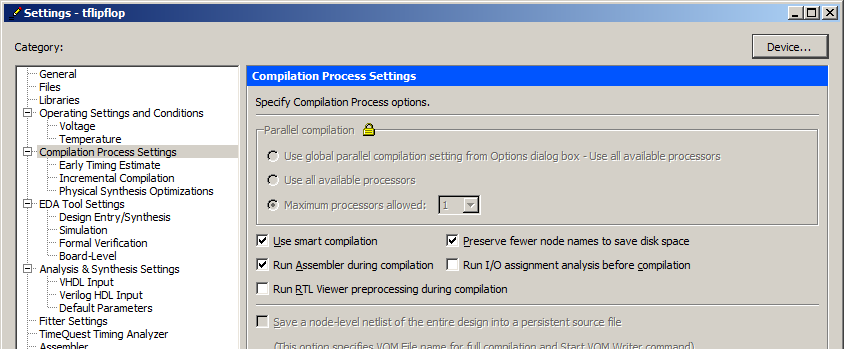
\includegraphics[scale=\tutpicscale]{225smartcompilation.png}
\caption{Instellen van van de optie Smart compilation.}
\label{fig:225smartcompilation}
\end{figure}


\section{Quartus blijft hangen}
\label{sec:quartusblijfthangen}
Er is een aantal situaties waardoor Quartus blijft hangen en alleen maar
via de Task Manager van Windows kan worden afgesloten. Hieronder de lijst met
bekende problemen:

\begin{itemize}\itemsep-1pt
\item Bij het aanmaken van een nieuw project is als projectmap een map gekozen
      waar je als gebruiker geen schrijfrechten voor hebt. Een mooi voorbeeld
      is de map \lstinline|C:\altera\13.0sp1|, de installatiemap van Quartus.
      Deze map wordt standaard opgegeven bij het aanmaken van een nieuw
      project. De oplossing is uiteraard eenvoudig: selecteer een andere map.
\item De bestanden van het project staan opgeslagen op de H:-schijf. Soms is
      deze schijf tijdelijk niet beschikbaar, bijvoorbeeld als gevolg door
      veel gebruikers. De oplossing: gewoon even wachten, na een tijdje
      reageert Quartus weer.
\end{itemize}

\fi


\section{Ingestelde pad naar ModelSim wordt niet opgeslagen}
\label{sec:ingesteldepadnaarmodelsimwordtnietopgeslagen}
Het is een paar keer gebleken dat, ondanks dat het pad naar de ModelSim
executable ingesteld is, ModelSim niet gestart kan worden. Dit komt vooral
voor bij versie 13.1 van Quartus. Het is mogelijk om handmatig een
verwijzing in te stellen naar de ModelSim executable.

\begin{itemize}\itemsep-1pt
\item Open de map waar het gebruikersprofiel is opgeslagen, meestal iets in
      de trant van \lstinline|C:\Users\<gebruikersnaam>|
\item Open het initialisatie-bestand \lstinline|quartus2.ini|
\item Voeg de volgende code toe, uiteraard met de juiste padnaam
\begin{lstlisting}[language=VHDL,numbers=none,belowskip=-3.5ex]
[EDA_Tool_Paths 13.1]
EDA_TOOL_PATH_MODELSIM_ALTERA = C:\altera\13.1\modelsim_ae\win32aloem
\end{lstlisting}
\item Sluit het bestand
\item Start Quartus opnieuw op

\end{itemize}


\section{Gebruik USB-Blaster onder Linux}
\label{sec:gebruikvanusbblasteronderlinux}
Als je onder Linux als gewone gebruiker inlogt, kan je niet direct gebruik
maken van de USB-aansluiting. Je krijgt dan een foutmelding zoals te zien is
in figuur \ref{fig:230jtagerror89}.

%\begin{itemize}\itemsep-1pt
%\item[] \lstinline|Unexpected error code 0x89, operation failed.|
%\end{itemize}

\begin{figure}[H]
\centering
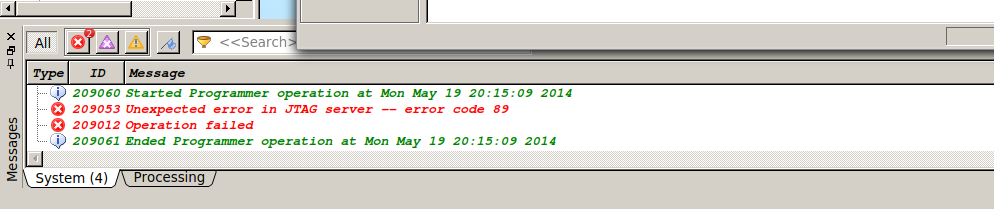
\includegraphics[scale=\tutpicscale]{231Aquartus_errorCode_89}
\caption{Foutmelding bij programmeren onder Linux.}
\label{fig:230jtagerror89}
\end{figure}

Voer de volgende handelingen uit om als gewone gebruiker de USB-Blaster te
kunnen gebruiken. De handelingen zijn getest op CentOS 6.5. De handelingen
moet je als gebruiker \lstinline|root| uitvoeren.

\begin{itemize}\itemsep-1pt
\item Maak een bestand \lstinline|40-usbblaster.rules| aan in de map
      \lstinline|/etc/udev/rules.d|
\item Plaats in het bestand de volgende code (let hierbij goed op het afbreken
      van de regels):
\begin{lstlisting}[language=VHDL,numbers=none,belowskip=-3.5ex]
# USB-Blaster

SUBSYSTEM=="usb", ENV{DEVTYPE}=="usb_device", ATTRS{idVendor}=="09fb", ATTRS{idProduct}=="6001", MODE="0666", SYMLINK+="usbblaster/%k"
SUBSYSTEM=="usb", ENV{DEVTYPE}=="usb_device", ATTRS{idVendor}=="09fb", ATTRS{idProduct}=="6002", MODE="0666", SYMLINK+="usbblaster/%k"
SUBSYSTEM=="usb", ENV{DEVTYPE}=="usb_device", ATTRS{idVendor}=="09fb", ATTRS{idProduct}=="6003", MODE="0666", SYMLINK+="usbblaster/%k"

# USB-Blaster II
SUBSYSTEM=="usb", ENV{DEVTYPE}=="usb_device", ATTRS{idVendor}=="09fb", ATTRS{idProduct}=="6010", MODE="0666", SYMLINK+="usbblaster2/%k"
SUBSYSTEM=="usb", ENV{DEVTYPE}=="usb_device", ATTRS{idVendor}=="09fb", ATTRS{idProduct}=="6810", MODE="0666", SYMLINK+="usbblaster2/%k"
\end{lstlisting}
\item Sluit het bestand
\item Herlees de udev-regels met \lstinline|udevadm control --reload-rules|
\item Trigger de updates met \lstinline|udevadm trigger|
\item Herstart de progammer-software
\end{itemize}


%\section{Design Rule S102}
%\label{sec:designrules102}
%Als je de melding \lstinline|S102: Synchronous Port and Asynchronous Port of the Same Register Should Not Be Driven by the Same Signal Source|
%krijgt, heb je waarschijnlijk een asynchrone \'{e}n synchrone reset in je
%ontwerp gebruikt. Zoek alle deelontwerpen af naar deze twee vormen en verander
%alle synchrone resets in asynchrone resets. Zie
%\url{http://quartushelp.altera.com/13.0sp1/mergedProjects/verify/da/comp_file_rules_synch_reset.htm}
%en klik op de \textsl{buttons} om de schema's te openen.


\section{Bestandsnaam en entity-naam}
\label{sec:bestandsnaamenentitynaam}
Een \textsl{entity} is een hardware-eenheid en levert bij synthese
dus hardware op. Een \textsl{bestandsnaam} is de naam van het bestand
waarin de hardware beschreven of getekend is. De entity-naam is
onafhankelijk van het gebruikte besturingssysteem, de bestandsnaam is
wel afhankelijk.

In Quartus zijn schemabestanden met de extensie \naam{.bdf}
gekoppeld aan de entity-naam: de bestandsnaam zonder de extensie
is gelijk ook de entity-naam.

Bij beschrijvingstalen als VHDL en Verilog ligt dat anders: de
bestandsnaam hoeft niet hetzelfde te zijn als de entity-naam. In feite
is het bestand een \textsl{container} met daarin de beschrijving
van de hardware. ModelSim gebruikt de bestandsnaam om de beschrijving
te compileren (bv.\@ met \naam{vcom} en \naam{vlog}) maar gebruikt de
entity-naam bij het starten van de simulatie (m.b.v.\@ \naam{vsim}).

Het is raadzaam om de bestandnaam (zonder extensie) hetzelfde te houden
als de entity-naam. Daarmee voorkom je problemen.

Let op: entity-namen mogen \textsl{niet} beginnen met een cijfer of
een leesteken. In feite gelden voor de entity-namen dezelfde regels als
voor variabelen. Schemabestandsnamen mogen dus ook niet met een cijfer
of een leesteken beginnen, VHDL-bestandsnamen wel.


\section{Opruimen van een Quartus-project}
\label{sec:opruimenvaneenquartusproject}
Quartus heeft de neiging om tijdens compilatie ontzettend veel, vooral kleine
bestanden aan te maken. Je kan heel veel van die bestanden en mappen gewoon
verwijderen als je project is afgerond.

De mappen \lstinline|db|, \lstinline|incremental_db|, \lstinline|output_files|
en \lstinline|simulation| kan je gewoon verwijderen. Let erop dat je geen
eigen aangemaakte bestanden in de map \lstinline|simulation| moet hebben staan.

Onderstaand script kan je draaien in een Windows-command box en verwijdert
bijna elk bestand dat niet nodig is (de bovengenoemde mappen met inhoud
moet je eerst zelf verwijderen).

\begin{lstlisting}[caption=Windows opruimscript,label=cod:opruim]
@echo off
rem
rem
echo.
echo This program will delete all unnessecary files from Quartus projects.
echo.
echo Please be VERY carefull! Press Ctrl-C to break.
echo.
pause
echo.

del /s *.done
del /s *.rpt
del /s *.sof
del /s *.pof
del /s *.summary
del /s *.jdi
del /s vsim.wlf
del /s *.bak
del /s transcript
del /s *assignment_defaults.qdf
del /s *.pin
del /s modelsim.ini
del /s *.qws
del /s *.smsg
del /s *.map
del /s *.cdf
del /s *.dpf

echo.
echo Done.
echo.
pause
\end{lstlisting}

%\section{Pinnen worden niet getoond in de Pin Planner}
%Als de pinnen niet worden getoond in de Pin Planner, heb je waarschijnlijk
%geen \textsl{Device Type} opgegeven en staat het type op \textsl{Auto}. Ga
%via menu \menu{Assignments\pijl{}Device} en vul de juiste gegevens in.
%Zie ook figuur~\ref{fig:028familydevicesettings}.
%
%\section{Verkeerde pinnen worden getoond}
%Dan heb je de verkeerde entity als top-level ingesteld. Zie
%paragraaf~\ref{sec:fouttoplevel}.

%\section{ModelSim stopt na enige tijd}
%Als ModelSom na enige tijd stopt voordat de simulatie werkelijk gestart
%wordt, dan ben je vergeten om de do-file op te geven. Zie de figuren
%\ref{fig:074assignmentssettings} en \ref{fig:073settingssimulation}.
%



\appendix

\chapter{Knoppen en sneltoetsen}
\label{chap:knoppenensneltoetscombinatie}
In deze bijlage is een tabel opgenomen met een aantal knoppen en
sneltoetscombinaties. Niet alle knoppen worden in deze tutorial gebruikt.

%\newcolumntype{V}{>{\centering\arraybackslash} m{3cm} }

\begin{table}[H]
%\renewcommand\arraystretch{1.0}
\caption{Knoppen en sneltoetscombinaties.}
\label{tab:knoppenensneltoetscombinaties}
\centering
\begin{tabular}[t]{|c|p{4.5cm}|p{6.5cm}|l|}
\hline
& & & \\[-2ex]
\textbf{Knop} & \textbf{Benaming} & \textbf{Menu} & \textbf{Sneltoets} \\ [0.7ex] \hline
\parbox[c][2.5em]{2em}{\includegraphics[scale=1]{112viewprojectnavigator}} & View Project Navigator & \vspace*{-17pt}\naam{View\pijl{}Utility Windows\pijl{}Project Navigator} & Alt+0 \\ \hline
\parbox[c][2.5em]{2em}{\includegraphics[scale=1]{111device}} & Device Assignments & \naam{Assignments\pijl{}Device} & - \\ \hline
\parbox[c][2.5em]{2em}{\includegraphics[scale=1]{113settings}} & Settings Assignments & \naam{Assignments\pijl{}Settings} & Ctrl+Shift+E \\ \hline
\parbox[c][2.5em]{2em}{\includegraphics[scale=1]{114assignmenteditor}} & Assignment Editor* & \naam{Assignments\pijl{}Editor} & Ctrl+Shift+A \\ \hline
\parbox[c][2.5em]{2em}{\includegraphics[scale=1]{115pinplanner}} & Pin Planner & \naam{Assignments\pijl{}Pin Planner} & Ctrl+Shift+N \\ \hline
\parbox[c][2.5em]{2em}{\includegraphics[scale=1]{116floorplanner}} & Floor Planner* & \naam{Tools\pijl{}Chip Planner} & - \\ \hline
\parbox[c][2.5em]{2em}{\includegraphics[scale=1]{117startcompilation}} & Start Compilation & \naam{Processing\pijl{}Start Compilation} & Crtl+L \\ \hline
\parbox[c][2.5em]{2em}{\includegraphics[scale=1]{118startanalysisandsynthesis}} & Start Analysis & \vspace*{-17pt}\naam{Processing\pijl{}Start\pijl{}Start Analysis \& Synthesis} & Crtl+K \\ \hline
\parbox[c][2.5em]{2em}{\includegraphics[scale=1]{119startiminganalyser}} & \vspace*{-17pt}Start TimeQuest Timing Analyser* & \vspace*{-17pt}\naam{Processing\pijl{}Start\pijl{}Start TimeQuest Timing Analyser} & Ctrl+Shift+T \\ \hline
\parbox[c][2.5em]{2em}{\includegraphics[scale=1]{120timinganalyser}} & \vspace*{-17pt}Open TimeQuest Timing Analyser* & \vspace*{-17pt}\naam{Tools\pijl{}TimeQuest Timing Analyser} & - \\ \hline
\parbox[c][2.5em]{2em}{\includegraphics[scale=1]{121rtlsimulation}} & RTL Simulation & \vspace*{-17pt}\naam{Tools\pijl{}Run Simulation Tools\pijl{}RTL Simulation} & - \\ \hline
\parbox[c][2.5em]{2em}{\includegraphics[scale=1]{122gatelevelsimulation}} & Gate Level Simulation* & \vspace*{-17pt}\naam{Tools\pijl{}Run Simulation Tools\pijl{}Gate Level Simulation} & - \\ \hline
\parbox[c][2.5em]{2em}{\includegraphics[scale=1]{123compilationreport}} & Compilation Report & \naam{Processing\pijl{}Compilation Report} & Crtl+R \\ \hline
\parbox[c][2.5em]{2em}{\includegraphics[scale=1]{124programmer}} & Programmer & \naam{Tools\pijl{}Programmer} & - \\ \hline
\parbox[c][2.5em]{2em}{\includegraphics[scale=1]{125analysecurrentfile}} & Analyse Current File & \vspace*{-17pt}\naam{Processing\pijl{}Analyse Current File} & - \\ \hline
\parbox[c][2.5em]{2em}{\includegraphics[scale=1]{126inserttemplate}} & Insert Template & \naam{Edit\pijl{}Insert Template} & - \\ \hline
\end{tabular}
\end{table}
\vskip-4ex
* Wordt niet gebruikt tijdens deze tutorial.


\chapter{Pinbenaming EP3C16F484C-6N}
\label{chap:pinbenaming}
In deze bijlage vind je de pinbenaming terug. Er staan ook opmerkingen bij.

\begin{table}[H]
\centering
\caption{Pinbenamingen FPGA, deel 1.}
\label{tab:pinbenamingenfpga1}
\begin{tabular}[t]{|p{3cm}|p{3cm}|p{2cm}|p{5cm}|}
\hline 
\rb{Type}         & \rb{Quartus-naam} & \rb{Pinnaam} & \rb{Opmerking} \\ \hline 
                  &                &          &   \\  \hline 
\rb{Clock}        & \rb{CLOCK\_50} & \rb{G21} & \rb{Global Clock 1} \\  \hline 
                  &                &          &   \\  \hline 
\rb{Push Buttons} & \rb{BUTTON[0]} & \rb{H2}  & \rb{Ontdenderd, actief laag} \\  \hline 
                  & \rb{BUTTON[1]} & \rb{G3}  &   \\  \hline 
                  & \rb{BUTTON[2]} & \rb{F1}  &   \\  \hline 
                  &                &          &   \\  \hline 
\rb{Switches}     & \rb{SW[0]}     & \rb{J6}  & \rb{Niet ontdenderd, actief hoog} \\  \hline
                  & \rb{SW[1]}     & \rb{H5}  &  \\  \hline
                  & \rb{SW[2]}     & \rb{H6}  &  \\  \hline
                  & \rb{SW[3]}     & \rb{G4}  &  \\  \hline
                  & \rb{SW[4]}     & \rb{G5}  &  \\  \hline
                  & \rb{SW[5]}     & \rb{J7}  &  \\  \hline
                  & \rb{SW[6]}     & \rb{H7}  &  \\  \hline
                  & \rb{SW[7]}     & \rb{E3}  &  \\  \hline
                  & \rb{SW[8]}     & \rb{E4}  &  \\  \hline
                  & \rb{SW[9]}     & \rb{D2}  &  \\  \hline
                  &                &          &   \\  \hline 
\rb{Leds}         & \rb{LEDG[0]}   & \rb{J1}  & \rb{Actief hoog} \\ \hline
                  & \rb{LEDG[1]}   & \rb{J2}  & \\ \hline
                  & \rb{LEDG[2]}   & \rb{J3}  & \\ \hline
                  & \rb{LEDG[3]}   & \rb{H1}  & \\ \hline
                  & \rb{LEDG[4]}   & \rb{F2}  & \\ \hline
                  & \rb{LEDG[5]}   & \rb{E1}  & \\ \hline
                  & \rb{LEDG[6]}   & \rb{C1}  & \\ \hline
                  & \rb{LEDG[7]}   & \rb{C2}  & \\ \hline
                  & \rb{LEDG[8]}   & \rb{B2}  & \\ \hline
                  & \rb{LEDG[9]}   & \rb{B1}  & \\ \hline
\end{tabular} 
\end{table}
\vspace*{-2ex}
Dit zijn de benamingen zoals ze in de documentatie van het DE0-bordje worden
gebruikt. Je kan ook je eigen namen gebruiken. Quartus zal, wanneer van
toepassing, het woord \naam{PIN\_} voor de pinnaam zetten, dus J2 wordt dan 
\naam{PIN\_J2}.

Op de volgende pagina staan de pingegevens van de 7-segment displays. Tevens
is de layout gegeven.

\newpage
\begin{table}[H]
\centering
\caption{Pinbenamingen FPGA, deel 2.}
\label{tab:pinbenamingenfpga2}
\begin{tabular}{|m{3cm}|m{3cm}|m{2cm}|m{5cm}|}
\hline 
\rb{Type}      & \rb{Quartus-naam} & \rb{Pinnaam} & \rb{Opmerking} \\ \hline 
               &                   &              &   \\  \hline 
\rb{7-segment} & \rb{HEX0\_D[0]}   & \rb{E11}     & \rb{Alle actief laag} \\  \hline
               & \rb{HEX0\_D[1]}   & \rb{F11}     &  \\  \hline
               & \rb{HEX0\_D[2]}   & \rb{H12}     &  \\  \hline
               & \rb{HEX0\_D[3]}   & \rb{H13}     &  \\  \hline
               & \rb{HEX0\_D[4]}   & \rb{G12}     &  \\  \hline
               & \rb{HEX0\_D[5]}   & \rb{F12}     &  \\  \hline
               & \rb{HEX0\_D[6]}   & \rb{F13}     &  \\  \hline
               & \rb{HEX0\_DP}     & \rb{D13}     &  \\  \hline
               &                   &              &   \\  \hline 
               & \rb{HEX1\_D[0]}   & \rb{A13}     &  \\  \hline
               & \rb{HEX1\_D[1]}   & \rb{B13}     &  \\  \hline
               & \rb{HEX1\_D[2]}   & \rb{C13}     &  \\  \hline
               & \rb{HEX1\_D[3]}   & \rb{A14}     &  \\  \hline
               & \rb{HEX1\_D[4]}   & \rb{B14}     &  \\  \hline
               & \rb{HEX1\_D[5]}   & \rb{E14}     &  \\  \hline
               & \rb{HEX1\_D[6]}   & \rb{A15}     &  \\  \hline
               & \rb{HEX1\_DP}     & \rb{B15}     &  \\  \hline
               &                   &              &   \\  \hline 
               & \rb{HEX2\_D[0]}   & \rb{D15}     &  \\  \hline
               & \rb{HEX2\_D[1]}   & \rb{A16}     &  \\  \hline
               & \rb{HEX2\_D[2]}   & \rb{B16}     &  \\  \hline
               & \rb{HEX2\_D[3]}   & \rb{E15}     &  \\  \hline
               & \rb{HEX2\_D[4]}   & \rb{A17}     &  \\  \hline
               & \rb{HEX2\_D[5]}   & \rb{B17}     &  \\  \hline
               & \rb{HEX2\_D[6]}   & \rb{F14}     &  \\  \hline
               & \rb{HEX2\_DP}     & \rb{A18}     &  \\  \hline
               &                   &              &   \\  \hline 
               & \rb{HEX3\_D[0]}   & \rb{B18}     &  \\  \hline
               & \rb{HEX3\_D[1]}   & \rb{F15}     &  \\  \hline
               & \rb{HEX3\_D[2]}   & \rb{A19}     &  \\  \hline
               & \rb{HEX3\_D[3]}   & \rb{B19}     &  \\  \hline
               & \rb{HEX3\_D[4]}   & \rb{C19}     &  \\  \hline
               & \rb{HEX3\_D[5]}   & \rb{D19}     &  \\  \hline
               & \rb{HEX3\_D[6]}   & \rb{G15}     &  \\  \hline
               & \rb{HEX3\_DP}     & \rb{G16}     &  \\  \hline
\end{tabular}                      
\end{table}                         
\vspace*{-2.0ex}                    
\begin{figure}[H]
\centering
\includegraphics[scale=0.25]{004layout7seg.png}
\caption{Layout 7-segment displays}
\label{fig:004layout7seg}
\end{figure}



\chapter{INLDIG-flow onder Linux}
\label{chap:inldigflowonderlinux}
Tijdens het practicum wordt gebruik gemaakt van een eigen \textsl{flow}.
In een flow staan de handelingen die door Quartus gedaan moeten worden om
tot het gewenste resultaat te komen. Deze flow is nodig voor het uitvoeren
van de practicumopdrachten. 

Er is echter een probleem: ModelSim kan alleen maar VHDL-code (en Verilog)
simuleren. Er is een script gemaakt (\lstinline|start_sim.tcl|) dat alle
\naam{.bdf}-bestanden vertaalt naar VHDL-code en vervolgens de simulator
start. Het script is zo geschreven dat het ook op Windows draait.

Om de flow op Linux te laten draaien moet je de volgende handelingen
verrichten:

\begin{itemize}\itemsep-1pt
\item Installeer de Quartus-software op een standaard plaats, bijvoorbeeld
      \lstinline|/opt/bin/|
\item Installeer de Modelsim-software\footnote{Vanaf versie 13.0 wordt
      ModelSim automatisch mee-ge\"{\i}nstalleerd.} onder de Altera-root
      (met versienummer), meestal iets van \lstinline|/opt/bin/altera/13.0sp1/| 
\item Download het bestand \lstinline|inldig_common_tutorial.zip |van
      BlackBoard of de website\\ \url{http://ds.opdenbrouw.nl/quartus/} 
\item Pak het bestand uit in een map, bijvoorbeeld
      \naam{/home/\textsl{username}/QUARTUS/INLDIG}. Je krijgt dan twee
      mappen genaamd \naam{common} en \naam{tutorial}
\end{itemize}

Kopieer het bestand \lstinline|tmwc_INLDIG_Compile_And_Simulation.tmf| in de
direcory \naam{common} naar de directory
\naam{/home/\textsl{username}/.quartus.altera}.
Als je die directory niet hebt, moet je \'{e}\'{e}n keer Quartus starten of
zelf aanmaken. Wijzig het pad onderin het bovengenoemde bestand naar de
juiste locatie. \textbf{Let op: geen spaties in de padnaam!} Als
voorbeeld is een pad van de gebruiker \naam{jesse} opgenomen. 

\bigskip
\begin{lstlisting}[numbers=none]
... beginstuk weggelaten ...
    <task> 
        <id>Start Simulation</id> 
        <name>Start Simulation</name> 
        <item_bitmap>tcl_command</item_bitmap> 
        <status_ok_if>project_is_open</status_ok_if> 
        <action type =
            "tcl_command">/home/jesse/QUARTUS/INLDIG/common/start_sim.tcl</action> 
    </task> 
</tasks> 
\end{lstlisting}



\chapter{INLDIG-flow onder Windows}
\label{chap:inldigflowonderwindows}
Tijdens het practicum wordt gebruik gemaakt van een eigen \textsl{flow}.
In een flow staan de handelingen die door Quartus gedaan moeten worden om
tot het gewenste resultaat te komen. Deze flow is nodig voor het uitvoeren
van de practicumopdrachten. 

Er is echter een probleem: ModelSim kan alleen maar VHDL-code (en Verilog)
simuleren. Er is een script gemaakt (\lstinline|start_sim.tcl|) dat alle
\naam{.bdf}-bestanden vertaalt naar VHDL-code en vervolgens de simulator
start. Het script is zo geschreven dat het ook op Linux draait.
 
Om de flow op Windows te laten draaien moet je de volgende handelingen
verrichten:

\begin{itemize}\itemsep-1pt
\item Installeer de Quartus-software op een standaard plaats, bijvoorbeeld
      \lstinline|c:\altera\|.
\item Installeer de Modelsim-software\footnote{Vanaf versie 13.0 wordt
      ModelSim automatisch mee-ge\"{\i}nstalleerd.} onder de Altera-root
      (met versienummer), meestal iets van \lstinline|c:\altera\13.0sp1\| 
\item Download het bestand \lstinline|inldig_common_tutorial.zip |van
      BlackBoard of de website\\ \url{http://ds.opdenbrouw.nl/quartus/}. 
\item Pak het bestand uit in een map, bijvoorbeeld
      \lstinline|D:\QUARTUS\INLDIG\|. Je krijgt dan twee mappen genaamd
      \lstinline|common| en \lstinline|tutorial|
\end{itemize}
      
De flow is opgeslagen onder de naam
\lstinline|tmwc_INLDIG_Compile_And_Simulation.tmf| in de map \lstinline|common|
en moet ge\"{\i}nstalleerd worden in de \textsl{profile map} van de gebruiker,
meestal iets van\\ \lstinline|C:\Users\<gebruikersnaam>\| (natuurlijk zonder
$<$ en $>$).

Om nu de flow onder Windows te gebruiken moet je de padnaam in het bovengenoemde
bestand wijzigen in de juiste locatie.
\textbf{Let op: geen spaties in de padnaam!}

\bigskip
\begin{lstlisting}[numbers=none]
... beginstuk weggelaten ...

    <task> 
        <id>Start Simulation</id> 
        <name>Start Simulation</name> 
        <item_bitmap>tcl_command</item_bitmap> 
        <status_ok_if>project_is_open</status_ok_if> 
        <action type =
            "tcl_command">D:/QUARTUS/INLDIG/common/start_sim.tcl</action> 
    </task> 
</tasks> 
\end{lstlisting}

\end{document} 
